\documentclass[12pt,english]{article}

\newif\ifblind
\blindfalse

\usepackage[utf8]{inputenc}
\usepackage{tgpagella}
\usepackage{mathpazo}
\usepackage[margin=1.3in]{geometry}
\usepackage[round,sort&compress]{natbib}
\usepackage{url}
\usepackage{tcolorbox}
\usepackage[hyperpageref]{backref}
\usepackage[pagebackref]{hyperref}
\hypersetup{
  colorlinks=true,
  urlcolor=purple,
  linkcolor=blue,
  citecolor=violet,
}
\usepackage{amsmath,amssymb,amsthm,mathtools}
\usepackage{babel}
\usepackage{graphicx}
\usepackage{caption}
\usepackage{subcaption}
\usepackage{booktabs}
\usepackage{threeparttable}
\usepackage{gensymb}
\usepackage{textcomp}
\usepackage{setspace}
\usepackage{lineno}
\usepackage{placeins}
\setcitestyle{aysep={}}

\newtheorem{proposition}{Proposition}
\newtheorem{corollary}{Corollary}
\theoremstyle{remark}
\newtheorem*{remark}{Remark}

\title{International Transfers or\\Differentiated Carbon Prices?}

\ifblind
  \author{}
  \date{}
\else
\renewcommand{\url}[1]{\href{#1}{Link}}

  \author{Adrien Fabre\thanks{CNRS; CIRED. Corresponding author: adrien.fabre@cnrs.fr.} \and Constance Gorge\thanks{CIRED.} \thanks{We thank Marie Young-Brun and her co-authors for sharing the NICE model and for their advice.
  We received funding from the Agence Nationale de la Recherche (ANR-24-CE03-7110). We have no conflict of interest to disclose.}}
  \date{\today}
\fi

\begin{document}

\maketitle
\ifblind\else
  \begin{center}
    \textbf{\href{https://github.com/bixiou/NICE2020/raw/main/cap_and_share/paper/paper.pdf}{Link to most recent version}}
  \end{center}
\fi

\begin{abstract}
\noindent Recent proposals for international carbon pricing differentiate national carbon prices by income. The usual justification is that cross-border transfers are politically infeasible. But differentiated prices are themselves equivalent to transfers. We show that any schedule of national prices is distributionally equivalent to a uniform price combined with a certain allocation of tradable emission rights, equal, to first order, to each country's emissions under autarky.
In a dynamic setting, the equivalent rights are weighted by the discounted carbon price, and under Hotelling pricing they reduce to a carbon budget. Because abatement costs are convex, this allocation leaves every country weakly better off, so the uniform price with equivalent rights Pareto-dominates autarky.
We quantify the equivalence in NICE, an integrated assessment model with 179 countries.
Replacing the schedules of \citet{parry_proposal_2021}, \citet{wolfram_building_2025}, or \citet{banerjee_grand_2025} with a uniform price and equivalent rights would cut the coalition's emissions by 4--5\% while leaving every member as well off. Alternatively, holding emissions fixed, it would raise every member's consumption by 0.05--0.06\%, half the implicit transfers of differentiation: differentiation loses about half a dollar of consumption for every dollar of implicit transfer.
We also review the departures from standard assumptions that could justify price differentiation and argue that they are less compelling than often thought.
\end{abstract}

\medskip
\noindent\textbf{Keywords:} carbon pricing; international climate agreements; emissions trading; burden sharing; differentiated carbon prices; international transfers; integrated assessment.

\noindent\textbf{JEL:} Q54; Q58; H23; F53; D61.

\clearpage

\ifblind
  \doublespacing
  \linenumbers
\else
  \tableofcontents
\fi

\section{Introduction}
\label{sec:intro}

International climate policy is stuck on a distributional question: who should obtain the rights to emit? The Paris Agreement endorses common but differentiated responsibilities and respective capabilities, and it commits developed countries to financing climate action in developing ones. It does not translate these principles into numbers, and national contributions remain far short of its temperature goal \citep{unep_emissions_2025}.

A prominent recent answer is to coordinate carbon prices while differentiating them by income. The IMF proposes an international price floor of \$75, \$50 and \$25/tCO$_2$ for high-, upper middle- and lower-income countries \citep{parry_proposal_2021}. \citet{wolfram_building_2025} propose a climate coalition built on the same tiers. \citet{banerjee_grand_2025} propose a ``grand bargain'' in which low- and middle-income countries adopt prices of \$10 to \$50/t in exchange for compensation for their climate damages. In all three proposals, carbon revenues are retained domestically. Differentiation is meant to deliver equity without the cross-border transfers that are deemed politically infeasible \citep{parry_proposal_2021}.

Textbook theory prescribes something else: a uniform price for efficiency, and lump-sum transfers for equity \citep{aldy_promise_2012}. Differentiated prices are a second-best substitute for transfers, and the case for income-based differentiation therefore rests on the premise that transfers are infeasible. This paper argues that the premise does not rest on solid ground. Survey evidence already challenges it: majorities accept an international carbon price financing North--South transfers in all 23 surveyed countries \citep{fabre_majority_2025,fabre_public_2025}.
Furthermore, a uniform price can achieve efficiency while remaining
distributionally equivalent to differentiated prices. We make the claim precise in three results.

First, any schedule of differentiated autarky prices is distributionally equivalent to a uniform price combined with a specific allocation of tradable emission rights. To first order, this allocation grants each country the emissions it has under autarky. A country allowed a price below the uniform price therefore receives more rights than it emits at the uniform price, and sells the difference.
Conversely,  positive price gap is equivalent to less emission rights.
In a static setting, we derive
a second-order formula for equivalent rights in terms of the price gap and the price elasticity of emissions (Proposition~\ref{prop:equiv}).\footnote{We use the terms \textit{rights} and \textit{allocation} interchangeably: while \textit{rights} refers to a cap-and-trade framework, our analysis equally applies to revenue \textit{allocation} in a carbon tax.}

Second, granting each country its emissions under the schedule leaves every country weakly better off under the uniform price than under autarky (Proposition~\ref{prop:dominance}). This is the familiar gains-from-trade logic of emissions markets \citep{montgomery_markets_1972}, which \citet{fleurbaey_when_2025} also apply to differentiated prices at a fixed cap, and the international analogue of production efficiency \citep{diamond_optimal_1971}. Its implication for the policy debate is less familiar: any price-differentiation agreement can be replaced by a uniform price with an allocation of rights such that no country loses. The resulting surplus can take the form of reduced emissions or of increased consumption.

Third, in a dynamic setting the equivalence holds in present value, with each year's rights weighted by the discounted carbon price (Proposition~\ref{prop:dynamic}). When the carbon price follows a Hotelling path, the equivalent allocation is a carbon budget: each country's cumulative emissions under autarky.

We quantify the equivalence in NICE \citep{young-brun_within-country_2025}, an integrated assessment model with 179 countries,
in two exercises.
First, for eight diverse economies, we compare aggregate consumption (or welfare) under a differentiated autarky price and under a global uniform price with a given allocation, holding global emissions on a path that exhausts a carbon budget of 1000\,GtCO$_2$ over 2025--2100. For each autarky price
and each allocation, we compute the welfare difference and trace the indifference
curve between the two regimes.
The curves show that the equivalence runs only one way: many allocations of rights, including an equal per capita allocation, cannot be replicated by any schedule of non-negative prices, because a zero price is not enough to compensate low emitters. For example, Nigeria prefers a uniform price to any non-negative autarky price, including a zero price, as long as its rights per capita are at least 25\% of the global average.

Second, we compute the equivalent rights for prominent differentiated-price proposals.
Granting all members their equivalent rights cuts coalition emissions by 3.9\% \citep{banerjee_grand_2025}, 4.8\% \citep{wolfram_building_2025,parry_proposal_2021}
and 13.4\% \citep{equal_right_climate_2023}, while leaving every member's consumption as high as under the schedule. Alternatively, the surplus raises every member's consumption by 0.05--0.06\% (0.19\% under Equal Right). These efficiency gains are about half the implicit transfers of differentiation: under the schedule of \citet{banerjee_grand_2025}, gross implicit transfers amount in present value to 0.11\% of the coalition's consumption, against an efficiency gain of 0.05\%. Differentiation thus loses about half a dollar of consumption for every dollar of implicit transfer.

We make three contributions. First, while the separation of efficiency and equity under lump-sum transfers and the gains from permit trading are well known \citep{chichilnisky_who_1994,montgomery_markets_1972,sandmo_global_2007}, and \citet{fleurbaey_when_2025} show that a common price is socially optimal when transfers or initial permit allocations can be freely adjusted,
we derive, in closed form, the correspondence from a given price schedule to the allocation of rights that reproduces its distributive outcome.
Second, we quantify the equivalence for actual proposals, including the implicit transfers of differentiation. Third, we find that, when revenues are pooled globally and returned to countries in proportion to population, as in \citet{equal_right_climate_2023},
differentiation leaves the lowest emitters worse off than a uniform price.

The remainder of the paper is organised as follows. Section~\ref{sec:arguments} reviews the rationales for differentiated carbon prices in a world that departs from standard assumptions. Section~\ref{sec:theory} derives the equivalence between differentiated prices and emission rights, in closed form in the static case and under additional assumptions in the dynamic case. Section~\ref{sec:by_country} uses NICE to trace, for seven major economies, the rights that leave each one indifferent to any given autarky price. Section~\ref{sec:proposals} computes the rights equivalent to prominent differentiated-price proposals, and the emissions cut or consumption gain obtained by replacing them with a uniform price. Section~\ref{sec:conclusion} concludes.

\section{Why differentiate carbon prices?}
\label{sec:arguments}

With complete markets and no other distortion,
efficiency requires a uniform carbon price, and equity should be addressed via lump-sum transfers \citep{sandmo_global_2007}.
Four departures from standard assumptions have been invoked to justify differentiating carbon prices across countries or sectors: divergent discount rates, pre-existing distortive taxes, market power in trade, and constraints on cross-country transfers. We review them in turn.

First, \citet{anthoff_differentiated_2026} show that equalising carbon prices across countries is inefficient in case of ``cross-country differences in discount rates (or interest rates)'', which arise from inefficiencies in the allocation of capital. By Hotelling's argument, each country's carbon price should grow at its own discount rate, so prices cannot be equal at all dates.\footnote{Differentiated prices may then be optimal in a second-best world, but the first best is in principle attainable by correcting the capital-market imperfections themselves.} The authors stress, however, that whether permit trade would then raise or lower welfare depends on its interaction with capital-market frictions, which no model has yet specified.

Second, pre-existing tax distortions can be mitigated by differentiating carbon prices across sectors or countries \citep{babiker_is_2004,boeters_optimally_2014}. For example, if aviation remains under-taxed, a higher carbon price on aviation than on other sectors improves welfare. Applying this logic to countries, \citet{babiker_is_2004} show that a uniform price is not necessarily beneficial to the countries that take part in it. However, \citet{dautume_should_2016} show that a uniform price remains optimal if the other tax (such as a gasoline tax) addresses a local externality or if public goods have to be funded by distortive taxation.

Third, large countries have market power in world markets, which gives them a terms-of-trade motive to differentiate \citep{babiker_climate_2005,boeters_optimally_2014}. Take China, a large oil importer and manufacturing exporter.
By taxing oil more heavily than other goods, China would depress world oil demand and hence the oil price, improving its terms of trade. Similarly, it has an interest in setting a higher carbon price on manufactured goods, to raise the price of its exports (to the extent that the carbon price paid by importers outweighs the exports lost to higher prices).

Fourth, and most commonly, differentiated prices are justified by the assertion that international transfers are politically infeasible \citep{parry_proposal_2021,young-brun_within-country_2025}. \citet{bauer_quantification_2020} describe an ``efficiency--sovereignty'' trade-off in climate policy: either carbon prices are differentiated and efficiency is lost, or a uniform price with transfers is applied, hampering national sovereignty. This reasoning assumes that international transfers constitute a stronger infringement on sovereignty than coordinated price differentiation \citep[see also][]{bekkers_comparing_2022}. \citet{fleurbaey_when_2025} formalise it: when transfers are ruled out or permit endowments are fixed, differentiated prices, including within a carbon market, can be efficient and socially preferable to a uniform price.
The first three rationales have an efficiency basis and do not rest on the absence of transfers. They also call for a differentiation that bears no systematic relation to income: by discount rate, by sector or by market power. This paper addresses the fourth rationale, the one invoked by differentiation proposals. We show that it cannot rest on the distributional implications of transfers, since differentiation is equivalent to transfers of the same size as those that a uniform price with equivalent rights would involve.

\paragraph{Related literature.}
Our analysis builds on the literature that evaluates specific differentiated price floors.
In a global general equilibrium model, \citet{chateau_global_2024} find that the IMF's international carbon price floor \citep{parry_proposal_2021} achieves higher welfare than a uniform price \textit{without transfers} attaining the same emission reductions (at \$56/t), since it shifts part of the mitigation effort from low- to high-income countries.
\citet{he_analysis_2024} show that, relative to national pledges, the IMF price floors bind on developing countries such as China and India but not on high-income countries, which makes the arrangement unattractive to developing countries.

\citet{le_moigne_distributional_2026} find that income-differentiated floors do not necessarily yield fairer outcomes. Compared with a uniform tax accompanied by the North--South transfers that equalise costs across countries (\$107--169 billion a year), all variants of the IMF floor entail larger global real-income losses, and most of them require larger transfers to reach the same fairness. We provide the first mapping from such schedules to equivalent allocations of emission rights.

Our results also speak to the literature on negotiating a common carbon price or a global cap-and-trade with revenue sharing \citep{grubb_greenhouse_1990,weitzman_can_2014,gollier_negotiating_2015,cramton_global_2017,nordhaus_climate_2015,fabre_global_2024}. The equivalence
formula gives climate negotiators a closed-form  ``exchange rate'' between price
concessions and emission rights.
\section{The equivalence between differentiated prices and emission rights}
\label{sec:theory}

\subsection{Static setting}

Consider countries $i=1,\dots,I$ with populations $N_i$,
in a single period. Lower-case variables are per capita. Country $i$ emits $e_i$ at abatement cost $a_i(e_i)$, which is decreasing and convex in $e_i$. Facing a carbon price $p$, firms and households emit $e_i(p)$, optimising by equating the marginal abatement cost to (minus) the price: $a_i'(e_i(p)) = -p$. Consumption is
\begin{equation}
  c_i = y_i - a_i(e_i) + t_i,
\end{equation}
where $y_i$ is potential output and $t_i$ a net international transfer. Welfare is increasing in $c_i$ and decreasing in global emissions through climate damages.

We compare two regimes that deliver the same global emissions $E=\sum_j N_j e_j$, whose world average per capita is $\bar e\equiv E/N$ (where $N$ is the world population).
Damages are then identical across regimes, and a country is better off in one regime if and only if its consumption is higher.

\paragraph{Autarky (differentiated prices).} Country $i$ applies a domestic price $p_i$, keeps its revenue and receives no transfer. It emits $e^A_i \equiv e_i(p_i)$, and $\sum_i N_i e^A_i = E$.

\paragraph{Uniform price.} The same countries apply a uniform price $p^*$ and trade emission rights under a cap equal to $E$.
Country $i$ receives rights $r_i$ per capita. At the market-clearing price, $\sum_i N_i e_i(p^*) = E$,
and $i$ emits $e^*_i \equiv e_i(p^*)$. Its net transfer is the value of its sales minus its purchases of rights, $t_i=(r_i-e^*_i)\,p^*$.

Throughout, a star denotes the uniform-price regime, a superscript $A$ the autarky regime and a bar a world average.
We write $\pi_i \equiv p_i/p^*$ for country $i$'s relative price, and $\varepsilon_i \equiv -\frac{p^*}{e^*_i}\,e_i'(p^*)$ for the price elasticity of its emissions at the uniform price. Define
\begin{equation}
  b_i \equiv a_i(e^A_i) - a_i(e^*_i) - a_i'(e^*_i)\,(e^A_i-e^*_i) \;\geq\; 0.
  \label{eq:bregman}
\end{equation}
$b_i$ is the deadweight loss of the price wedge $p_i - p^*$, i.e.\ the Harberger triangle of country $i$:
the area enclosed by the country's marginal abatement cost curve, the horizontal line at $p^*$ and the vertical line at $e^A_i$.
Formally, $b_i$ is the Bregman divergence of $a_i$ between $e^A_i$ and $e^*_i$. It is non-negative by convexity, and strictly positive if $a_i$ is strictly convex and $p_i\neq p^*$.

Denote by $r^*_i$ the \textit{equivalent rights} that leave country $i$ exactly as well off under the uniform-price regime as under the autarky regime with a price $p_i$.
\begin{proposition}[Equivalent rights]\label{prop:equiv}
Holding total emissions at $E$ and the carbon price at $p^*$, we have
\begin{equation}
  r^*_i \;=\; e^A_i - \frac{b_i}{p^*}.
  \label{eq:req_exact}
\end{equation}

To first order in the price gap,
\begin{equation}
  r^*_i \approx e^A_i \approx e^*_i\Bigl[\,1+\varepsilon_i(1-\pi_i)\Bigr].
    \label{eq:req_first}
\end{equation}
To second order, with $\varepsilon_i$ evaluated at $p^*$,
\begin{equation}
  r^*_i \;\approx\; e^A_i - \frac{(e^A_i-e^*_i)^2}{2\,\varepsilon_i\,e^*_i}
  \;\approx\; e^*_i\Bigl[\,1+\varepsilon_i(1-\pi_i)-\tfrac12\,\varepsilon_i(1-\pi_i)^2\Bigr].
  \label{eq:req_second}
\end{equation}
\end{proposition}

\begin{proof}
Equating $y_i-a_i(e^*_i)+(r_i-e^*_i)p^*$ with $y_i-a_i(e^A_i)$ gives $r_i=e^*_i+[a_i(e^*_i)-a_i(e^A_i)]/p^*$. Substituting $a_i'(e^*_i)=-p^*$ into \eqref{eq:bregman} yields \eqref{eq:req_exact}. Equation \eqref{eq:req_first} follows from $e^A_i-e^*_i\approx\varepsilon_i e^*_i(1-\pi_i)$. For \eqref{eq:req_second}, note that $a_i''(e^*_i)=-1/e_i'(p^*)=p^*/(\varepsilon_i e^*_i)$, so that $b_i\approx \tfrac12\,p^*\,(e^A_i-e^*_i)^2/(\varepsilon_i e^*_i)$.
\end{proof}

Proposition~\ref{prop:equiv} shows that a differentiated price is equivalent to a transfer paid in kind. Relative to the uniform price, a country allowed a lower price ($\pi_i<1$) keeps emissions $e^A_i>e^*_i$. To first order, the uniform-price regime replicates its situation by granting it exactly those emissions as rights, part of which it then sells, receiving $(e^A_i-e^*_i)p^*$. Conversely, a country asked for a higher price ($\pi_i>1$) is in the position of a country that buys rights. The size of the implicit transfer grows with the price gap, the country's emissions and the elasticity of those emissions. The same formula, read in reverse, converts any allocation of rights into an equivalent autarky price.

It is convenient to express an allocation as a multiple of the world average, $r_i=\rho_i\,\bar e$, so that $\rho_i=1$ is an equal per capita allocation. We denote by $\rho^*_i\equiv r^*_i/\bar e$ the equivalent ratio, and by $\hat\rho_i$ its first-order approximation:
\begin{equation}
  \hat\rho_i \;\equiv\; \frac{e^A_i}{\bar e},
  \label{eq:rhohat_static}
\end{equation}
country $i$'s per capita emissions under the differentiated schedule relative to the world average. By \eqref{eq:req_exact}, $\rho^*_i=\hat\rho_i-b_i/(p^*\bar e)\le\hat\rho_i$: the first-order prediction errs on the generous side. A differentiated schedule is thus, to first order, a grandfathering rule, applied to the emissions that the schedule itself induces.

\begin{proposition}[Dominance of the uniform price]\label{prop:dominance}
Allocate rights $r_i=e^A_i$ to every country. This allocation (i) is feasible at the cap of the autarky regime, $\sum_i N_i r_i=E$; (ii) leaves every country weakly better off than under the autarky regime
if $a_i$ is convex;
and (iii) leaves a surplus of $\sum_i N_i b_i\geq 0$. Expressed in emissions, the rights can be cut
to the equivalent allocation $(r^*_i)_i$, with no country worse off than under differentiated prices.
\end{proposition}

\begin{proof}
Part (i) holds by construction. For part (ii), the consumption gain of country $i$ is $[a_i(e^A_i)-a_i(e^*_i)]+(e^A_i-e^*_i)p^*=b_i\geq0$. For part (iii), sum these gains.
\end{proof}

A country that is allowed a lower price saves on abatement costs.
Under the uniform price, the same country can abate up to $p^*$ and sell the freed rights at $p^*$, which is always at least as good a deal. By Proposition~\ref{prop:equiv}, the surplus is of second order in the price gaps, whereas the implicit transfers are of first order. The ratio of the two therefore grows with price dispersion: the larger a schedule's price gaps, the more consumption it loses per dollar of implicit transfer.

The equivalent rights $r^*_i$ of Proposition~\ref{prop:equiv} leave country $i$ indifferent at a fixed price $p^*$. Turning the surplus into a lower cap raises the price, so that the rights $\tilde r_i$ that leave every country indifferent at the reduced cap and at the price it induces, with ratio $\tilde\rho_i\equiv\tilde r_i/\bar e$, are slightly greater than $r^*_i$. Therefore, the attainable emissions cut differs from $\sum_i N_i b_i/p^*$; we solve for it, and for $\tilde\rho_i$, numerically in Section~\ref{sec:proposals}.

Proposition~\ref{prop:dominance} is a first-best statement that abstracts from the second-best rationales for differentiation reviewed in Section~\ref{sec:arguments}, none of which requires the absence of transfers.
What it questions is the argument that differentiation is needed because transfers would be infeasible: differentiation has the same distributive outcome as well-chosen transfers; it only makes them implicit.

\subsection{Dynamic setting}
\label{sec:dynamic}

With several periods, variables become trajectories indexed by $t$, and $\beta_t$ denotes the discount factor. Under total utilitarianism, country $i$'s objective is $\sum_t \beta_t\,N_{it}\,c_{it}$.
It is therefore convenient to state the dynamic results in totals rather than per capita, denoted by upper-case letters: $R_{it}\equiv N_{it}r_{it}$ and $E_{it}\equiv N_{it}e_{it}$ are country $i$'s rights and emissions in period $t$, $E^A_{it}$ its emissions under the autarky regime, and $E_t=\sum_i E_{it}$ world emissions.

\begin{proposition}[Dynamic equivalence]\label{prop:dynamic}
Suppose abatement costs are separable over time. To first order in the price gaps $p_{it}-p^*_t$, country $i$ is indifferent between the autarky regime and the uniform price path $(p^*_t)$ with rights $(R_{it})$ if and only if
\begin{equation}
  \sum_t \beta_t\,p^*_t\,\bigl(R_{it}-E^A_{it}\bigr) \;=\; 0.
  \label{eq:dyn_equiv}
\end{equation}
If rights are a constant multiple $\rho_i$ of an equal per capita share, $r_{it}=\rho_i\,\bar e_t$,
the equivalent ratio is, to first order,
\begin{equation}
  \hat\rho_i \;=\; \frac{\sum_t \beta_t\,p^*_t\,N_{it}\,e^A_{it}}{\sum_t \beta_t\,p^*_t\,N_{it}\,\bar e_t}:%
  \label{eq:rhohat_dyn}
\end{equation}
the country's emissions under autarky over its population share of world emissions, each period weighted by the discounted price.
\end{proposition}

\begin{corollary}[Hotelling case]\label{cor:hotelling}
If the discounted price $\beta_t p^*_t$ is constant over time, the dynamic equivalence \eqref{eq:dyn_equiv} only constrains cumulative rights $R_i\equiv\sum_t R_{it}$, which must equal the country's carbon budget under the autarky regime. If differentiated prices are homothetic, $p_{it}=\pi_i\,p^*_t$, this budget admits a first-order approximation as a function of the price ratio $\pi_i$, analogous to the static case:
\begin{equation}
  R_i \;\approx\; E^A_i \;\;\approx\; E^*_i\Bigl[\,1+\varepsilon_i(1-\pi_i)\Bigr],
  \label{eq:hotelling_budget}
\end{equation}
where $E^*_i\equiv\sum_t E^*_{it}$ (resp. $E^A_i\equiv\sum_t E^A_{it}$) denotes $i$'s cumulative emissions under the uniform price (resp. autarky), and $\varepsilon_i\equiv\sum_t \varepsilon_{it}E^*_{it}/E^*_i$ denotes the average over time, weighted by these emissions, of its price elasticities $\varepsilon_{it}$ at $p^*_t$. Consequently,
\begin{equation}
  \hat\rho_i \;=\; \frac{E^A_i}{\sum_t \frac{N_{it}}{N_t}\,E_t},
  \label{eq:rhohat_hotelling}
\end{equation}
that is, the ratio of country $i$'s share of the cumulative emissions under autarky to its equal per capita share of the world carbon budget.
\end{corollary}

\begin{proof}
Apply the first-order argument of Proposition~\ref{prop:equiv} period by period. In period $t$ the consumption gain per capita is $p^*_t(r_{it}-e^A_{it})$ to first order; under total utilitarianism it enters the country's objective multiplied by its population, which turns per capita quantities into totals,
and it is discounted by $\beta_t$. Summing over $t$ and setting the total to zero gives \eqref{eq:dyn_equiv}. Substituting $R_{it}=\rho_i(N_{it}/N_t)E_t$ into \eqref{eq:dyn_equiv} gives \eqref{eq:rhohat_dyn}, and $\beta_t p^*_t$ cancels from it when it is constant, leaving \eqref{eq:rhohat_hotelling}. Likewise, a constant $\beta_t p^*_t$ factors out of \eqref{eq:dyn_equiv}, which then reads $\sum_t (R_{it}-E^A_{it})=0$. If $p_{it}=\pi_i p^*_t$, then \eqref{eq:req_first} applied in each period gives $E^A_{it}\approx E^*_{it}[1+\varepsilon_{it}(1-\pi_i)]$, and summing over $t$ gives \eqref{eq:hotelling_budget}.
\end{proof}

Proposition~\ref{prop:dynamic} and Corollary~\ref{cor:hotelling} assume that international transfers do not alter future state variables such as the capital stock; NICE, in which transfers affect investment and growth, therefore extends them quantitatively beyond this setting.

Equation~\eqref{eq:dyn_equiv} shows that timing matters. A tonne of rights is worth more in a period of high (discounted) prices, so the allocation depends on the whole price path, and a country's cumulative carbon budget does not by itself determine its welfare.
With a constant carbon price, the discounted price falls over time, and countries whose emissions fall quickly under autarky need more rights than their cumulative share suggests, because the discounted price is higher in the short term when their emissions are high.
Only under a Hotelling price path, the natural benchmark with a fixed carbon budget and efficient capital markets, does the price weighting drop out, and \eqref{eq:hotelling_budget} then states that a differentiated price is worth to a country the domestic carbon budget it induces. Because rights are defined as a per capita multiple rather than a share of global emissions, equation~\eqref{eq:rhohat_hotelling} also carries a demographic correction.

\section{Equivalent rights by country}
\label{sec:by_country}
\label{sec:model}

\subsection{Model}

We use NICE \citep{young-brun_within-country_2025}, a recursive-dynamic integrated assessment model in the RICE tradition (itself an offshoot of DICE). It represents 179 countries, each disaggregated into income deciles with specific carbon footprints and climate damages, and is coupled to the FaIR climate model.
International transfers enter national income and therefore affect investment and subsequent growth.
Damages are country-specific: the damage function is applied to local temperatures.
All countries share the same cost function of the abatement rate
but differ only through their baseline emissions.
A given price therefore induces the same proportional abatement everywhere, so that the price elasticity $\varepsilon_i$ of Proposition~\ref{prop:equiv} is common to all countries at a given price, and cross-country differences in equivalent rights stem from differences in emissions and in autarky prices. Online Appendix~\ref{app:variants} gives further details.%

We present every result under two variants, which differ in how a country's situation is measured and in how carbon revenue is shared within it.
In the \emph{consumption} variant, we compare a country's situation in two regimes by the net present value over 2025--2100, discounted at 3\% a year, of its total consumption.
Domestic carbon revenues are recycled within each country in proportion to $c^{\eta}$, the inverse of marginal utility (Negishi weights, with $\eta=1.5$). This rule is our benchmark because it roughly preserves within-country inequality, which the criterion ignores, so that the comparisons isolate between-country effects.
In the \emph{welfare} variant, the criterion is the net present value of population-weighted equally-distributed-equivalent (EDE) consumption,\footnote{EDE consumption is the level of consumption which, equally distributed across deciles, would yield the same utilitarian welfare as the actual distribution.} with inequality aversion $\eta=1.5$, and revenues are returned as an equal per capita dividend within each country, which makes the domestic incidence of a carbon price progressive. Pricing carbon then reduces within-country inequality and can improve welfare even ignoring avoided climate damages, an effect that makes this variant unsuited to isolating the inefficiency of differentiated pricing.
We show the consumption variant in the main text, report the main figures of the welfare variant alongside, and give its full results in Online Appendix~\ref{app:eqpc}.

\subsection{Design}

The benchmark is an exponential uniform price path $p^*_t$, ramped up linearly from zero in 2025 over ten years and growing at a constant rate from 2036, which exhausts a carbon budget of 1000\,GtCO$_2$ over 2025--2100. Among such paths, we take the one that maximises discounted world welfare, damages included, over 2025--2300.\footnote{Welfare is discounted at a pure rate of time preference of 0.3\%, which, with $\eta=1.5$ and the model's 1.8\% annual growth of consumption per capita, corresponds to the 3\% discount rate on consumption used throughout.} The ramp-up reaches \$192/t in 2035, after which the price grows at 1.3\% a year, reaching \$229/t in 2050 and \$429/t in 2100. World emissions fall from 38\,GtCO$_2$ in 2025 to 27 in 2030, 20 in 2035 and 2 in 2100, and warming reaches 1.84\textdegree C in 2100.
The price grows more slowly than the 3\% discount rate, so that the discounted price falls over time: with damages in the objective, a tonne abated early is worth more than the carbon budget alone would imply.
For a given country $i$, we compare two scenarios with the same global emission path.

\begin{itemize}
  \item \emph{Autarky}: country $i$ applies $\pi_i p^*_t$ and recycles its revenue domestically. The rest of the world applies a uniform price that we solve for year by year so that global emissions stay on the path of the uniform-price run.
  \item \emph{Uniform price}: all countries apply $p^*_t$. Country $i$ receives rights per capita $\rho_i$ times its population share of global emissions in the same year, $r_{it}=\rho_i\,\bar e_t$,
  and the remaining rights go to the rest of the world in proportion to each country's emissions.
\end{itemize}

A grid over $(\pi_i,\rho_i)$ gives the net gain
between the two scenarios,
and hence country $i$'s indifference curve. We run the grid for seven diverse economies.

\subsection{Results}

Figure~\ref{fig:heatmaps} maps each country's consumption gain in the uniform-price regime relative to autarky over the $(\pi_i,\rho_i)$ plane, in the consumption variant; Figure~\ref{fig:heatmaps_eqpc} in Online Appendix~\ref{app:eqpc} is its welfare-variant analogue. Its indifference curve gives, for each autarky price factor, the smallest rights allocation at which the country prefers the uniform price. The first panel repeats the United States with the y-axis on a linear rather than a logarithmic scale: the curve is then close to a straight line, as equation~\eqref{eq:req_first} implies.

\begin{figure}[p]
  \centering
  \begin{subfigure}[b]{0.49\textwidth}\centering
    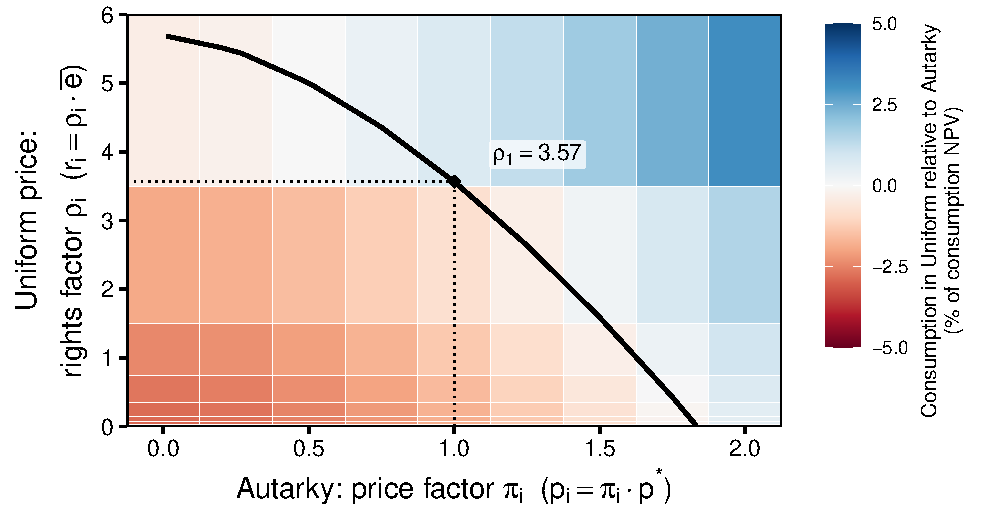
\includegraphics[width=\linewidth]{figures/heatmap_linear_USA.pdf}\caption{United States, linear y-axis}\end{subfigure}\hfill
  \begin{subfigure}[b]{0.49\textwidth}\centering
    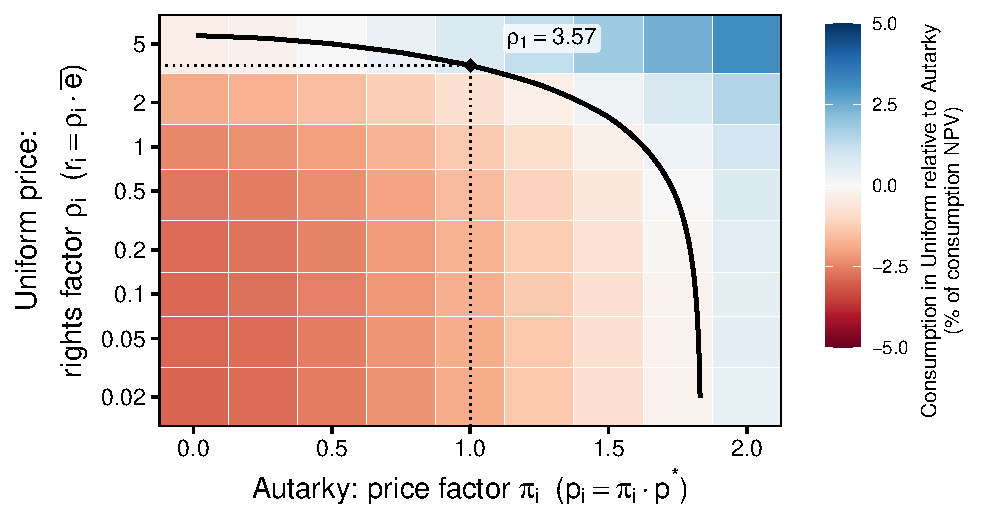
\includegraphics[width=\linewidth]{figures/heatmap_USA.pdf}\caption{United States}\end{subfigure}\\[2pt]
  \begin{subfigure}[b]{0.49\textwidth}\centering
    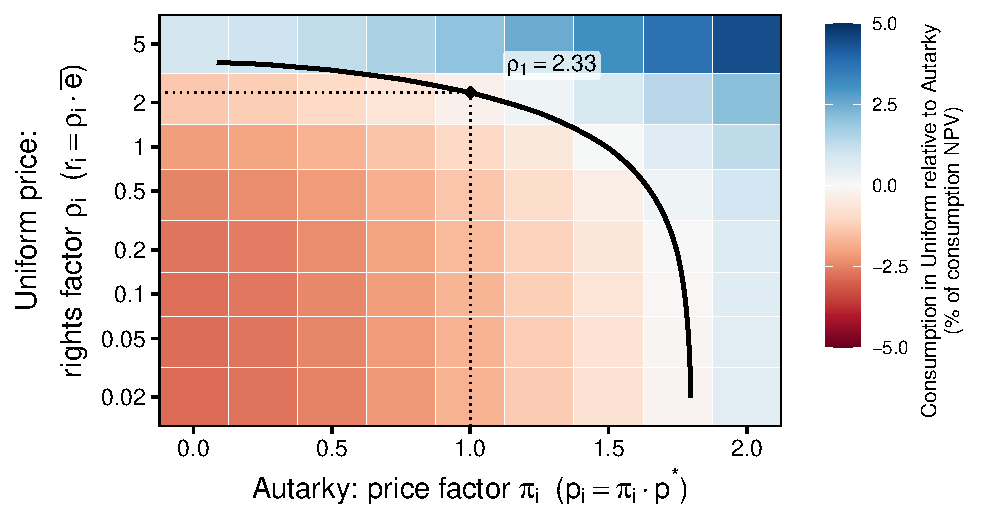
\includegraphics[width=\linewidth]{figures/heatmap_RUS.pdf}\caption{Russia}\end{subfigure}\hfill
  \begin{subfigure}[b]{0.49\textwidth}\centering
    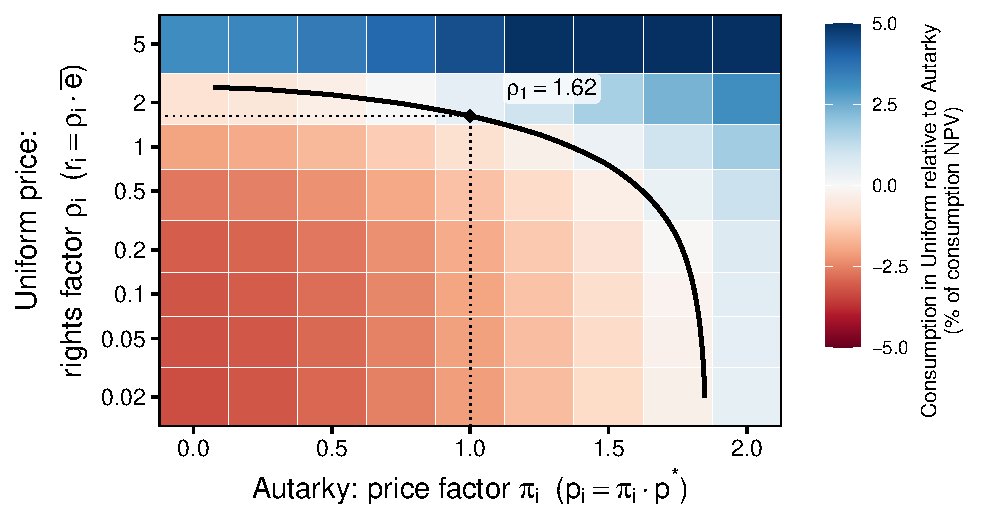
\includegraphics[width=\linewidth]{figures/heatmap_CHN.pdf}\caption{China}\end{subfigure}\\[2pt]
  \begin{subfigure}[b]{0.49\textwidth}\centering
    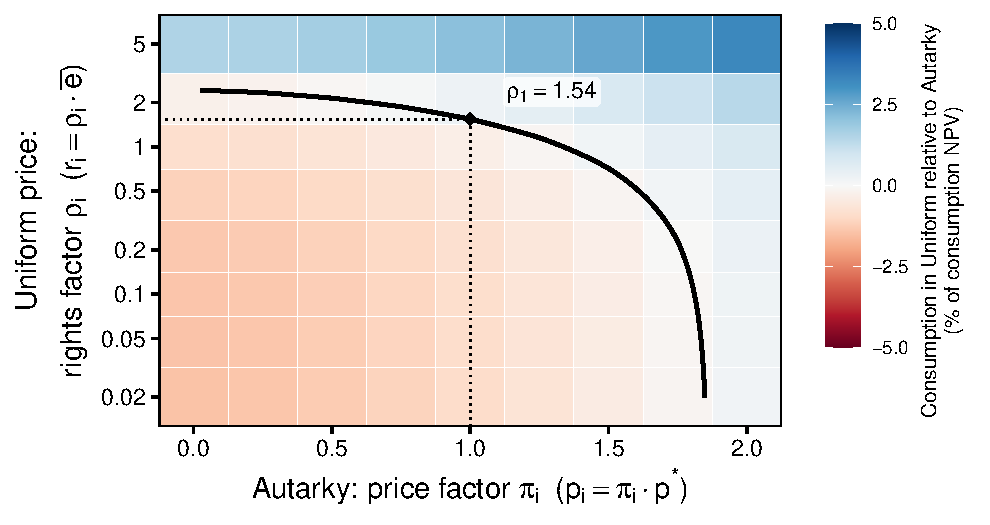
\includegraphics[width=\linewidth]{figures/heatmap_EU27.pdf}\caption{European Union (EU27)}\end{subfigure}\hfill
  \begin{subfigure}[b]{0.49\textwidth}\centering
    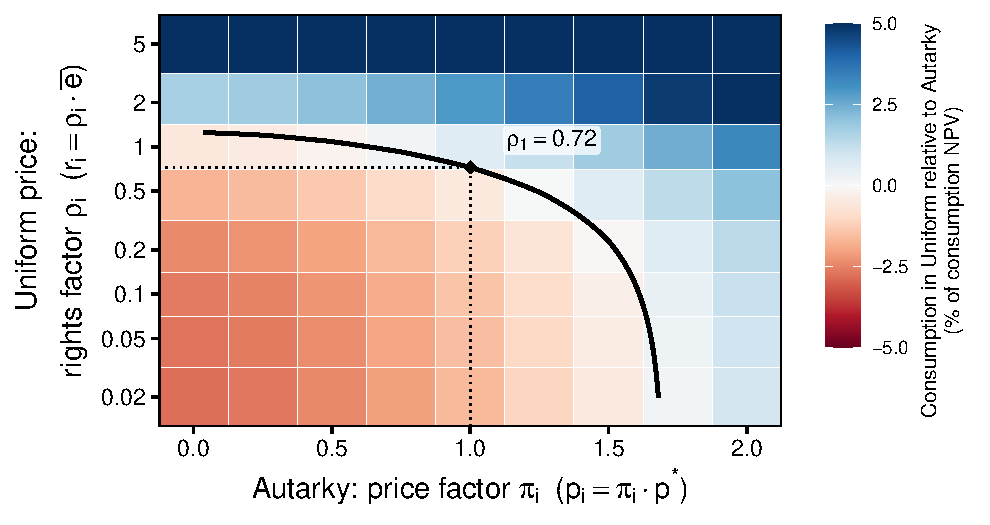
\includegraphics[width=\linewidth]{figures/heatmap_IND.pdf}\caption{India}\end{subfigure}\\[2pt]
  \begin{subfigure}[b]{0.49\textwidth}\centering
    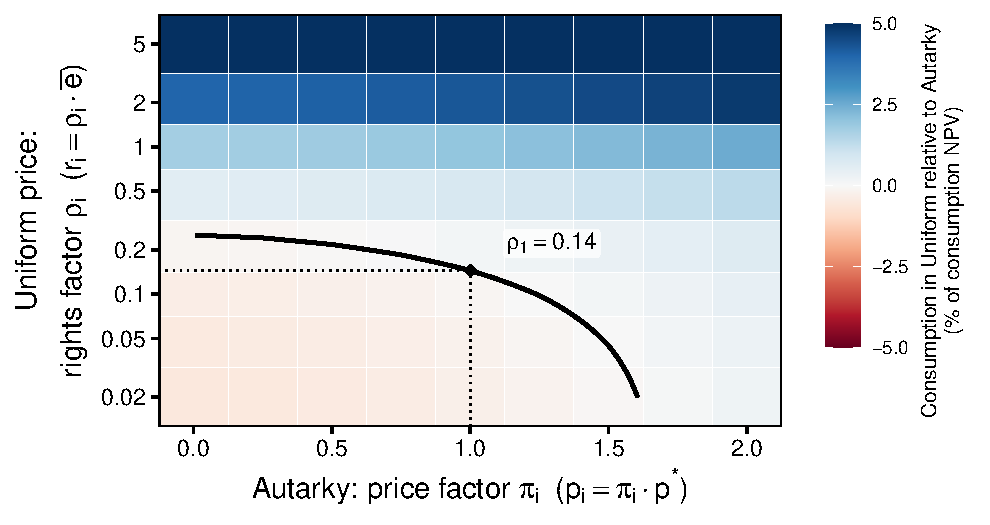
\includegraphics[width=\linewidth]{figures/heatmap_NGA.pdf}\caption{Nigeria}\end{subfigure}\hfill
  \begin{subfigure}[b]{0.49\textwidth}\centering
    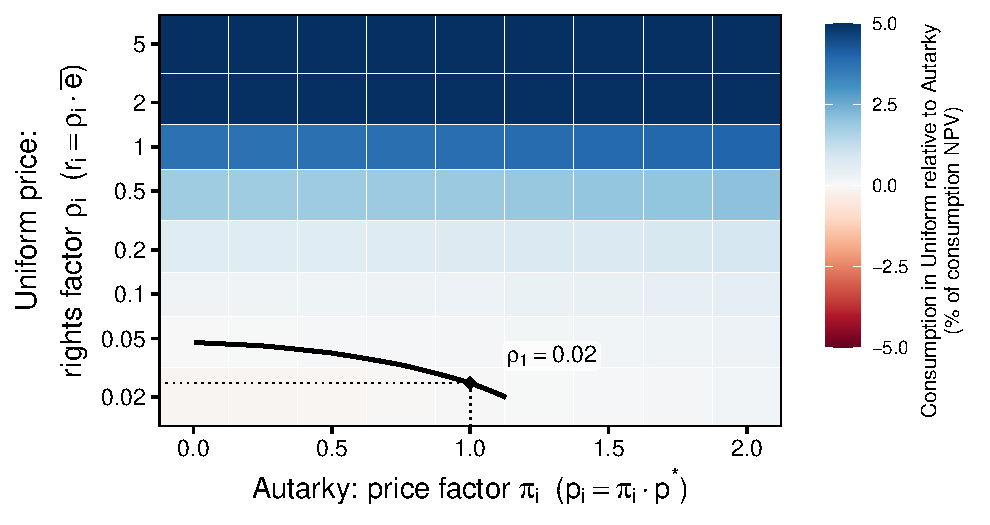
\includegraphics[width=\linewidth]{figures/heatmap_COD.pdf}\caption{DR Congo}\end{subfigure}
  \caption{Consumption gain of the uniform-price regime over autarky.}
  \label{fig:heatmaps}
  \begin{minipage}{\textwidth}\footnotesize\singlespacing
  \emph{Note}: The horizontal axis is country $i$'s autarky price as a multiple $\pi_i$ of the benchmark price $p^*_t$.
  The vertical axis is its allocation $\rho_i$ under the uniform price, as a multiple of world average emissions per capita: on a log scale in every panel but the first.
  Colours give the net gain in the uniform regime relative to autarky in terms of NPV of consumption over 2025--2100, in percent;
  blue cells are those where the uniform price is preferred to autarky. The black line is the indifference curve and $\rho_1$ its value at $\pi_i=1$. Global emissions are the same in both regimes at every point of the grid. Crosses mark allocations that would leave the rest of the world with negative rights.
  \end{minipage}
\end{figure}

\paragraph{Cumulative emissions predict equivalent rights.}
The intercept of each curve at $\pi_i=1$, denoted $\rho_1$, is consistent with the theory: when the autarky price equals the uniform price, the equivalent rights closely match the first-order approximation \eqref{eq:rhohat_dyn} based on the country's cumulative emissions (Table~\ref{tab:summary}).\footnote{The residual gaps are due to the homotheticity constraint on rights ($r_{it}=\rho_i \bar e$), which creates temporary price gaps that in turn trigger channels ignored by the first-order formula: the convexity of abatement costs, the effect of transfers on capital accumulation, and the within-country incidence of prices and transfers.}
Equivalent rights account for projected future emissions, which a 2025 snapshot does not.
In 2025, India emits 0.4 times the world average per capita, but it is equivalent to 0.72 shares, because its emissions hold up while the world's fall.
Conversely, the EU27, at 1.7 times the world average in 2025, is equivalent to 1.54 shares, because its emissions fall faster than the world's; China, at 1.5 times, is equivalent to 1.62 shares, because they fall more slowly.

\paragraph{Fair allocations cannot be replicated by differentiated prices.}
While every price schedule has an equivalent allocation, not every allocation has an equivalent non-negative price. At a zero price, a country cannot emit more than its unabated emissions, so this is the most that differentiation can offer.
For low emitters, that bound lies far below an equal per capita share: 0.28 for Nigeria and 0.05 for the DRC.
Burden-sharing principles that give such countries an equal per capita share or more --- as historical responsibility or capacity to pay would --- can only be achieved through a cap-and-trade or through monetary transfers.

\begin{table}[tbp]
\centering
\small
\singlespacing
\begin{threeparttable}
\caption{Allocation at which each country is indifferent when the autarky price equals the benchmark ($\pi_i=1$).}
\label{tab:summary}
\IfFileExists{../output/rho1_table.tex}{% Generated by src/indifference_curves.jl -- do not edit by hand.
\begin{tabular}{lrrrr}
  \toprule
  & Emissions p.c. & Emissions p.c. & Predicted & Simulated \\
  & in 2025 & in 2025 over & $\hat\rho_1$ & $\rho^*_1$ \\
  & (tCO$_2$) & world average & & \\
  \midrule
  United States & 17.65 & 3.77 & 3.56 & 3.57 \\
  Russia & 9.92 & 2.12 & 2.33 & 2.33 \\
  EU27 & 8.07 & 1.73 & 1.54 & 1.54 \\
  China & 7.22 & 1.54 & 1.62 & 1.62 \\
  Turkey & 4.86 & 1.04 & 1.33 & 1.33 \\
  India & 1.91 & 0.41 & 0.73 & 0.72 \\
  Nigeria & 0.59 & 0.13 & 0.15 & 0.14 \\
  DR Congo & 0.05 & 0.01 & 0.03 & 0.02 \\
  \bottomrule
\end{tabular}
}{}
\begin{tablenotes}\footnotesize
  \item \emph{Note}: $\hat\rho_1$ is equation~\eqref{eq:rhohat_dyn} evaluated on the uniform-price run: the country's emissions over its population share of world emissions, each year weighted by the discounted benchmark price over 2025--2100. $\rho_1$ is the value of the indifference curve in Figure~\ref{fig:heatmaps} at $\pi_i = 1$.
\end{tablenotes}
\end{threeparttable}
\end{table}

\section{Equivalent rights of prominent differentiation proposals}
\label{sec:proposals}

\subsection{Proposals}

We feed three proposals into the model as country-level price schedules.

\citet{wolfram_building_2025} envisage a coalition of 47 countries\footnote{The members are Algeria, Australia, Brazil, Cameroon, Canada, China, Egypt, the European Union, Ghana, Iceland, India, Indonesia, Kenya, Liechtenstein, Mozambique, Norway, Switzerland, Thailand, Togo, the United Kingdom, Uganda and Zambia.} including China, the EU, the UK, India and Brazil, which together emit 49\% of world CO$_2$ in 2030. Members apply \$75, \$50 and \$25/t in high-, upper-middle- and lower-income countries, the tiers of the IMF's international carbon price floor \citep{parry_proposal_2021}. The proposal targets four emissions-intensive industries, whereas NICE has no sectoral detail. We apply the floors economy-wide, so our scenario is more ambitious than the one the authors model.

\citet{banerjee_grand_2025} propose \$10, \$30 and \$50/t in low-, lower-middle- and upper-middle-income countries, in exchange for compensation for climate damages, with revenues retained domestically. High-income countries fund the compensation and are expected to price carbon heavily, but the proposal gives no figure. Rather than leaving them unpriced, we price them at \$75/t, the top tier of \citet{parry_proposal_2021} and \citet{wolfram_building_2025}.

\citet{equal_right_climate_2023} proposes a global system to phase out fossil fuel extraction that can be modelled as a schedule of differentiated prices.
Each country sells its extraction licences at a price graduated by income group (\$240, \$120, \$60 and \$30/t) and discounted by up to 60\% for climate vulnerability, which gives floors ranging from \$12 to \$240/t in 2025 (\$138/t on average, weighted by emissions), rising by about 16\% a year to stay within 1.5\textdegree C.
The revenues are pooled in a global fund that pays climate grants and a universal dividend. We model Equal Right's between-country transfers by returning global revenues to each country in proportion to its population.

The first two proposals do not specify how prices evolve over time. \citet{parry_proposal_2021} set their floors for 2030, \citet{wolfram_building_2025} simulate a single illustrative year and suggest ``sunset provisions that gradually raise lower-tier prices so countries `graduate' into a single uniform price'', and \citet{banerjee_grand_2025} raise a country's price only when it moves to a higher income group.
For each proposal, we hold the announced prices from 2025 through 2030 and raise them by 5\% a year thereafter, capped at the backstop price.
While \cite{wolfram_building_2025} and \citet{banerjee_grand_2025} include unquantified provisions to make prices converge, we do not model them, so as to compare differentiated prices with a cap-and-trade on clear terms. In Online Appendix~\ref{app:ede}, we also run Equal Right's original escalation path, which reaches the backstop in most countries by 2050.
The proposals yield a 2100 warming of 2.22\textdegree C \citep{wolfram_building_2025}, 1.87\textdegree C \citep{banerjee_grand_2025} and 1.67\textdegree C \citep{equal_right_climate_2023}.

\subsection{Design}

We compare each differentiation proposal with a cap-and-trade. Countries the proposal prices form a coalition whose members face a uniform price $p^*_t$, calibrated so that their joint emissions equal those under differentiation.
This price is \$51/t \citep{wolfram_building_2025}, \$56/t \citep{banerjee_grand_2025} and \$143/t \citep{equal_right_climate_2023} in 2030. It then grows by 4--5\% a year, slightly less than the 5\% of the schedules due to a composition effect: emissions shift towards the members with the lowest prices, which weigh more and more in the average price.
Non-members are unpriced in both regimes. Member $i$ receives rights per capita $r_{it}=\rho_i\,\bar e_t$, where $\bar e_t$ is the coalition's emissions per capita under the proposal, so that $\rho_i=1$ is an equal per capita allocation. This design differs from that of Section~\ref{sec:by_country} in two respects: the uniform price is not the benchmark path of Section~\ref{sec:by_country} but the coalition price that reproduces the proposal's emissions, and allocations are expressed relative to the coalition's emissions per capita rather than the world's.

We solve for the equivalent ratios in each of the two variants of Section~\ref{sec:model}: on the NPV of each member's total consumption, with Negishi recycling, and on the NPV of its EDE consumption, with an equal per capita dividend within countries (Online Appendix~\ref{app:eqpc}). Proposition~\ref{prop:dominance} implies that the coalition regime leaves a surplus, which we use in either of two ways:
\begin{itemize}
  \item \emph{Reduced emissions}: rights are cut (hence the price and abatement costs increase) until every member is as well off as under the proposal, which yields the ratios $\tilde\rho_i$ of Section~\ref{sec:theory}. This is our benchmark.
  As in Propositions~\ref{prop:equiv} and~\ref{prop:dominance}, members are compared at the same damages: while solving for the allocation, we hold each country's damages at the level implied by the proposal's own temperature path.\footnote{This is an accounting device used to isolate the efficiency gain of uniform pricing. If the price is below the social cost of carbon, accounting for avoided damages would tighten the cap past the social cost of carbon, until the extra abatement costs offset the climate benefits of the earlier cuts.
  Reduced emissions would then measure the ambition of a proposal rather than the instrument used to deliver it.}
  Once the rights are computed, we reintegrate avoided damages into the consumption (or welfare) gains we report.
  \item \emph{Increased consumption}: joint emissions are kept at their level under the proposal in every year, and the surplus rights are shared so as to maximise the smallest relative gain of any member, which equalises the gains of all members.
\end{itemize}
We solve each problem jointly for all members. At each iteration, the allocation sets the cap, the coalition price is recalibrated to deliver it, and each member's ratio is updated to improve the criterion. We iterate until convergence.
Online Appendix~\ref{app:variants} also reports two alternative ways of sharing the consumption surplus, and an \emph{isolated} solve, which finds each country's ratio in turn while every other member pays the coalition price and is granted its own emissions under the proposal as rights.

\subsection{Results}

Table~\ref{tab:equiv_rights_main} reports, for ten major economies, the allocation equivalent to each proposal, solved on consumption, together with the outcome of the two ways of using the surplus. For the schedule of \citet{banerjee_grand_2025}, it also reports the net transfer that the equivalent allocation implies.

\begin{table}[!ht]
\centering
\small
\singlespacing
\caption{Equivalent rights of three differentiated-price schedules, and the surplus of a uniform price.}
\label{tab:equiv_rights_main}
\resizebox{\textwidth}{!}{%
\IfFileExists{../output/equivalent_rights_main.tex}{% Generated by src/equivalent_rights_proposals.jl (write_main_table) -- do not edit by hand.
\begin{tabular}{lcccccccc}
  \toprule
  & \multicolumn{4}{c}{\textbf{Banerjee, Duflo \& Greenstone}} & \multicolumn{2}{c}{\textbf{Wolfram et al.}} & \multicolumn{2}{c}{\textbf{Equal Right, 5\%/yr}} \\
  \cmidrule(lr){2-5} \cmidrule(lr){6-7} \cmidrule(lr){8-9}
  \textbf{Country} & $p_{2030}$ & $\hat\rho$ & $\tilde\rho$ & $\tau$ (\%) & $p_{2030}$ & $\tilde\rho$ & $p_{2030}$ & $\tilde\rho$ \\
  \midrule
  United States & 75 & 2.63 & 2.51 & $-$0.39 & 0 & -- & 240 & $-$0.16 \\
  Russia & 75 & 1.71 & 1.61 & $-$0.38 & 0 & -- & 240 & 0.12 \\
  European Union (average) & 75 & 1.17 & 1.11 & $-$0.19 & 75 & 0.95 & 232 & 0.31 \\
  China & 50 & 1.61 & 1.60 & $-$0.02 & 50 & 1.39 & 108 & 1.13 \\
  Turkey & 50 & 1.28 & 1.29 & $-$0.03 & 0 & -- & 108 & 0.99 \\
  Indonesia & 50 & 0.90 & 0.91 & $-$0.05 & 50 & 0.77 & 96 & 0.91 \\
  Brazil & 50 & 0.41 & 0.41 & $-$0.02 & 50 & 0.36 & 108 & 0.78 \\
  India & 30 & 1.00 & 0.92 & 0.52 & 25 & 0.86 & 42 & 1.17 \\
  Nigeria & 30 & 0.21 & 0.19 & 0.09 & 0 & -- & 42 & 0.76 \\
  DR Congo & 10 & 0.08 & 0.05 & 0.12 & 0 & -- & 15 & 0.68 \\
  \midrule
  \multicolumn{9}{l}{\textit{Reduced emissions: every member as well off as under the proposal (ignoring avoided damages)}} \\
  World temp.~2100, change (\textdegree{}C) &  &  & $-$0.018 &  &  & $-$0.012 &  & $-$0.036 \\
  Emissions change in the coalition (\%) &  &  & $-$3.9\% &  &  & $-$4.8\% &  & $-$13.4\% \\
  Post-damage consumption gain (\%) &  &  & 0.029\% &  &  & 0.027\% &  & 0.095\% \\
  \midrule
  \multicolumn{9}{l}{\textit{Increased consumption: coalition emissions as under the proposal}} \\
  Coalition consumption gain (in \%) &  &  & 0.053\% &  &  & 0.059\% &  & 0.189\% \\
  \bottomrule
\end{tabular}
}{}%
}
\begin{minipage}{\textwidth}\footnotesize\singlespacing
\emph{Note}:
$p_{2030}$ is the price under differentiation.
$\tilde\rho$ is the country's equivalent rights as a multiple of the coalition's emissions per capita under differentiation, from the joint solve in its reduced-emissions form,
on the consumption criterion.
$\hat\rho$ is the first-order prediction of equation~\eqref{eq:rhohat_dyn}. $\tau$ is the implicit transfer that differentiation implies, i.e. the value of the country's net sales of rights at the coalition price, assuming its rights are its emissions under differentiation (in percent of its NPV of consumption).
Under Equal Right's proposal, revenue is pooled worldwide and returned in proportion to population, which is why its equivalent rights are so much lower for large per capita emitters and can even be negative.
The surplus of uniform pricing can be taken either as \emph{reduced emissions} or \emph{increased consumption}.
\end{minipage}
\end{table}
\FloatBarrier

\paragraph{The surplus as reduced emissions.} The uniform-price equivalent allocation of the Banerjee et al.\ differentiation reduces global emissions by 3.9\% and its 2100 warming by 0.02\textdegree C, while preserving pre-damage consumption in every country.
Reduced warming then makes every country better off than under differentiation, except for Mongolia, which would actually benefit from extra warming, according to our model:
it loses 0.01\% of its consumption, which could be compensated by extra rights amounting to 0.001\% of global 2025--2100 emissions.

The corresponding emission cuts are 4.8\% for \citet{wolfram_building_2025} and 13.4\% for the Equal Right schedule. In the welfare variant the cut is far larger (21\% for Banerjee et al.), but mostly because a higher coalition price funds a larger equal per capita dividend, whose redistribution within each member the welfare criterion values (Online Appendix~\ref{app:eqpc}).

\paragraph{The surplus as increased consumption.} Keeping emissions at their level under differentiation and sharing the surplus so as to equalise gains, every country gains 0.053\% of the net present value of its consumption vis-à-vis Banerjee et al.'s proposal.

\paragraph{The equivalent rights.}

For the Banerjee et al.\ schedule, the first-order prediction $\hat\rho_i$ of equation~\eqref{eq:rhohat_dyn} reproduces the solved allocations closely. As Proposition~\ref{prop:equiv} implies, it errs on the generous side for most countries, and by most for those priced furthest below the uniform price, whose second-order term is largest: 1.00 against 0.92 for India, 0.08 against 0.05 for the DRC.

The equivalent rights track the two determinants of Proposition~\ref{prop:equiv}: a country's emissions, and the gap between the price it is asked to apply and the coalition price of \$56/t.
The United States and Russia, priced at \$75/t and emitting well above the world average, need 2.51 and 1.61 shares; China, priced at \$50/t, needs 1.60; India, at \$30/t, 0.92; Nigeria, at the same price but emitting a quarter as much per capita, 0.19. The schedule of \citet{wolfram_building_2025} gives a similar picture among its 47 members. The Equal Right schedule, whose revenue does not stay at home, is a different matter.

\paragraph{The implicit transfers from differentiation.} Column $\tau$ of Table~\ref{tab:equiv_rights_main} gives the implicit transfers of the \citet{banerjee_grand_2025} schedule, $\tau_i \;=\; \sum_t \beta_t\,p^*_t\,(E^A_{it}-E^*_{it})$,
the present value of the rights country $i$ would sell (or buy) if granted its emissions under the schedule, expressed in percent to the present value of its consumption. They amount to $-0.39\%$ for the United States, $-0.02\%$ for China and $+0.52\%$ for India. Summed over the net recipients, the gross implicit transfers are 0.11\% of the coalition's consumption in present value, about twice the efficiency gain of 0.05\%.
Their yearly flow grows with the carbon price, from
  0.04\% of the coalition's consumption in 2030
to 0.12\%
in 2050,
when India receives 0.47\% of its consumption and the United States pays 0.41\% of its own.

\paragraph{A schedule with a global dividend.} Under Equal Right the carbon price revenue is pooled globally and returned to every country in proportion to population, so the equivalent allocation has to replace what the schedule charges a country \emph{and} what the fund pays it. To first order, a member is indifferent when $p^*_t R_{it} = p^*_t\,E^A_{it} + D_t\,N_{it}/N_t - p_{it}\,E^A_{it}$, with $D_t=\sum_j p_{jt}E^A_{jt}$ the world revenue and $p_{it}\,E^A_{it}$ the revenue forgone from domestic pricing.
Denoting by $\bar p_t \equiv D_t/E_t$ the average price paid under differentiation, the dividend is therefore worth not one equal per capita share but $\bar p/p^*$, about 0.65 under this schedule. This ratio is below one for two reasons. First, the allocation of Table~\ref{tab:equiv_rights_main} takes the surplus of uniform pricing as reduced emissions: the cap is 13.4\% below the schedule's emissions, so the coalition price is higher than the uniform price that would deliver the schedule's own emissions,
and in present value the latter is only 0.86 of the former. Second, there is a composition effect: at equal emissions, the members charged \$240/t abate almost everything, so that the tonnes that survive increasingly sit in the \$15--42/t tiers (most of them from the 2060s), and the emission-weighted mean price falls to 0.76 of the uniform price.

A member that emits almost nothing therefore has an equivalent rights ratio near $\bar p/p^*$ rather than one, which is why the DRC's ratio (0.68) is well below one. In the increased-consumption allocation, whose coalition price delivers the schedule's own emissions, only the composition effect remains and the DRC's ratio is 0.85. It remains below one, as does Nigeria's (0.97), whereas India (1.39), China (1.21) and Indonesia (1.13) are above one.
Counterintuitively, when revenue is pooled globally and returned equally, price differentiation thus leaves the lowest emitters worse off than a uniform price with equal per capita rights delivering the same emissions: the highest prices drive the high-income countries' emissions they apply to, and hence the revenue they raise for the fund, close to zero.

For six countries, the equivalent ratio is negative, e.g.\ $-0.16$ for the United States.
Matching the schedule then requires these countries to buy the rights to all their emissions and to pay a further sum, so that the equivalent of the schedule is a net payment rather than an allocation of rights. Net payments are what burden-sharing principles based on historical responsibility would call for \citep{fanning_compensation_2023}.

\FloatBarrier

\section{Conclusion}
\label{sec:conclusion}

Differentiating carbon prices by income is increasingly proposed as a way to reconcile carbon pricing with equity.
Yet a differentiated schedule is equivalent, to first order, to a uniform price with tradable rights that grandfather each country on the emissions the schedule itself induces. Differentiation is thus equivalent to transfers of the same first-order size, implicit in (excess or forgone) abatement rather than paid in money.
Moreover, since abatement costs are convex, the explicit version leaves every country better off.

Replacing the differentiated prices of \citet{wolfram_building_2025} or \citet{banerjee_grand_2025} with a uniform price at equivalent rights would cut the coalition's emissions by 4--5\%
while leaving every member as well off as under differentiation, and by 13\% under the more dispersed schedule of \citet{equal_right_climate_2023}. Alternatively, at unchanged emissions, it would raise every member's consumption, by 0.05--0.06\% for the first two schedules and 0.19\% for the third.
These efficiency gains may seem small, but they should be compared with the implicit transfers of differentiation. Under the schedule of \citet{banerjee_grand_2025}, the gross implicit transfers amount in present value to 0.11\% of the coalition's consumption, so that differentiation loses about half a dollar of consumption for every dollar of implicit transfer. The choice is therefore between implicit transfers, at that cost, and explicit transfers, which a uniform price with equivalent rights delivers without it.

The equivalence runs only one way. Every schedule of prices has an equivalent allocation of rights, but no schedule of non-negative prices can deliver to a low emitter what a generous allocation would: even a zero price leaves Nigeria below 30\% of an equal per capita share, and the DRC below 6\%.
Allocations based on equal per capita rights, historical responsibility or capacity to pay are therefore out of reach of price differentiation.

Two implications follow for negotiations. First, the equivalence formula provides a near-linear correspondence between a price and emission rights, allowing parties to shift the discussion from one notion to the other as needed.
Second, the value of national sovereignty invoked to dismiss an international cap-and-trade should be weighed against the efficiency gains of an international commitment.
Furthermore, survey evidence shows
that 85\% of respondents worldwide state that climate policy at the \textit{global} level is needed, at odds with the supposed taste for national sovereignty \citep{fabre_majority_2025}. Finally, robust majority acceptance of an international cap-and-trade funding equal per capita cash transfers indicates that most people are ready to accept large North--South transfers that differentiated autarky prices cannot deliver. Therefore, price differentiation might be justified only in a transition period towards an international cap-and-trade, as countries build up their administrative capacity.

The analysis has limitations. NICE has no capital market,
so it cannot capture the diverging capital return motive
for differentiation.
It has no sectoral detail, which forced us to apply sectoral proposals economy-wide and leaves out the country-specific costs of sectoral reallocation.
Extending the equivalence to settings with trade and different sectors, where a uniform price must coexist with border adjustments and territorial emissions can be distinguished from carbon footprints, is a natural next step to better inform climate negotiators.

\section*{Declaration of competing interest}
The authors declare no competing interests.

\section*{Data availability}

The code (Julia, built on the Mimi implementation of NICE) and all inputs needed to reproduce the results are publicly available on
\ifblind
[anonymised for review]
\else
% TODO: create this replication package's own repository, and replace the link below by it.
\href{https://github.com/bixiou/NICE2020/tree/main/cap_and_share}{github.com/bixiou/NICE2020}.
\fi

\section*{Declaration of generative AI use}
During the preparation of this work the authors used Claude Code (Opus 5) to assist with code and editing. The authors reviewed and edited the content and take full responsibility for it.

\singlespacing
\ifblind
  \bibliographystyle{plainnat}
\else
  \bibliographystyle{plainnaturl_clean}
\fi
\bibliography{price_rights}%

\clearpage
\appendix
\nolinenumbers
\setcounter{table}{0}
\renewcommand{\thetable}{A\arabic{table}}
\setcounter{figure}{0}
\renewcommand{\thefigure}{A\arabic{figure}}
\begin{center}\Large\bfseries Online Appendix\end{center}

\section{Solves, sharing rules, and model}
\label{app:variants}

Several modelling choices matter for the results: the price path under differentiation; the solve method (\textbf{\textit{joint}} or \textit{isolated}); the criterion (\textbf{\textit{consumption}} or \textit{welfare}); the within-country recycling (\textbf{\textit{Negishi}} or \textit{equal per capita}); the surplus sharing variant (\textbf{\textit{reduced emissions}}, surplus rights allocated \textit{to reach an equal increase in consumption}, \textit{in proportion to marginal utility}, or \textit{as a uniform rescaling of equivalent rights}). Our benchmark choices are in bold. Below, we report results for some of the alternatives and give further details on the model.

\paragraph{The two variants.} In the consumption variant, all runs use NICE with revenue recycling within each country in proportion to $c^{\eta}$, computed once from a uniform-price reference run and held fixed across runs; in the welfare variant, revenue is returned to each country's deciles in equal per capita amounts.
Both variants use the default income elasticity of emissions across deciles, emissions measured on a consumption basis (carbon footprints), and international transfers entering national income, hence investment. The same configuration is used in the differentiated and in the uniform-price regime, so that the two regimes differ only in prices and rights.

\paragraph{The two solves.} The \emph{joint} solve of the main text finds all $\rho_i$ at once (in its reduced-emissions form, the ratios $\tilde\rho_i$). At each iteration the allocation sets the cap, the coalition price is recalibrated to deliver it, and each member's ratio is moved by a secant step on its gap to the target. For the reduced-emissions variant, an outer loop then moves the level of the allocation until the members' common pre-damage gain is zero, so that every member ends exactly at its level under the schedule. The \emph{isolated} solve instead finds each country's ratio in turn, with every other member granted its own emissions under the schedule and the coalition price held at the value that reproduces the schedule's emissions. It is the partial-equilibrium counterpart of Proposition~\ref{prop:equiv}, and yields the fixed-price ratios $\rho^*_i$ rather than $\tilde\rho_i$: it ignores that the other members also change their allocation, and that the coalition price adjusts to the resulting cap.

The two solves nearly agree on the aggregate. Taking the equivalent allocation at face value cuts the Wolfram et al.\ coalition's emissions by 4.9\% (isolated) against 4.8\% (joint), and the Banerjee et al.\ coalition's by 4.1\% against 3.9\%. They differ on the distribution, and the difference is systematic.
Applied together, the isolated allocations add up to a tighter cap, which raises the uniform price: this raises every member's abatement costs and revalues the rights it trades, to the benefit of net sellers and the detriment of net buyers. The isolated allocations then leave 33 of 47 Wolfram et al.\ members and 39 of 179 Banerjee et al.\ members below their consumption level under the schedule, while the joint allocation leaves none, apart from the effect of avoided damages discussed below (Table~\ref{tab:equiv_rights}).

\paragraph{Alternative sharing rules.} The increased-consumption variant of the main text shares the surplus so as to maximise the smallest relative gain, which equalises the gains of all members. Two other rules are reported in Table~\ref{tab:equiv_rights}. Sharing the surplus in proportion to population times marginal utility directs it to the poorest members: it yields by far the largest inequality-averse gain (a world welfare gain of 0.241\% for Banerjee et al., against 0.053\% under the maximin rule) but, unlike the maximin rule, it leaves 9 of 179 members below their consumption under the schedule. Uniform scaling of the whole allocation is dominated: the extra rights go to the largest holders, and the looser cap lowers the coalition price, which devalues the rights of small, generously endowed net sellers. It leaves no member below on consumption, but its inequality-averse gain is the smallest of the three rules (0.045\% for Banerjee et al.), and 9 of 47 Wolfram et al.\ members and 64 of 179 Banerjee et al.\ members end below their welfare under the schedule.

\IfFileExists{../output/equivalent_rights_combined.tex}{% Generated by src/equivalent_rights_proposals.jl -- do not edit by hand.
\begin{table}[htbp]
\centering
\small
\caption{Club-price rights ratios $\rho_i$ equivalent to the Wolfram et al. and Banerjee, Duflo \& Greenstone proposals}
\renewcommand{\arraystretch}{1.15}
\resizebox{\textwidth}{!}{
\begin{tabular}{lcccccc}
  \toprule
  & \multicolumn{3}{c}{\textbf{Wolfram et al.}} & \multicolumn{3}{c}{\textbf{Banerjee, Duflo \& Greenstone}} \\
  \cmidrule(lr){2-4} \cmidrule(lr){5-7}
  \textbf{Country} & $p_i$ & $\rho^{\mathrm{isolated}}$ & $\rho^{\mathrm{joint}}$ & $p_i$ & $\rho^{\mathrm{isolated}}$ & $\rho^{\mathrm{joint}}$ \\
  \midrule
  United States & 0 & -- & -- & 75 & 2.49 & 2.51 \\
  Russia & 0 & -- & -- & 75 & 1.58 & 1.61 \\
  European Union & 75 & 0.90 & 0.95 & 75 & 1.10 & 1.11 \\
  China & 50 & 1.37 & 1.39 & 50 & 1.60 & 1.60 \\
  Turkey & 0 & -- & -- & 50 & 1.28 & 1.29 \\
  Indonesia & 50 & 0.76 & 0.77 & 50 & 0.90 & 0.91 \\
  Brazil & 50 & 0.36 & 0.36 & 50 & 0.41 & 0.41 \\
  India & 25 & 0.89 & 0.86 & 30 & 0.92 & 0.92 \\
  Nigeria & 0 & -- & -- & 30 & 0.19 & 0.19 \\
  DR Congo & 0 & -- & -- & 10 & 0.05 & 0.05 \\
  \midrule
  \multicolumn{7}{l}{\textit{Reduced emissions (variant 1)}} \\
  \textbf{\quad Emissions change in the coalition (\%)} &  & $-$4.9\% & $-$4.8\% &  & $-$4.1\% & $-$3.9\% \\
  \textbf{\quad World temp.~2100, change (\textdegree{}C)} &  & $-$0.013 & $-$0.012 &  & $-$0.019 & $-$0.018 \\
  \textbf{\quad World welfare gain (\%)} &  & 0.035\% & 0.029\% &  & 0.056\% & 0.055\% \\
  \textbf{\quad World consumption gain (\%)} &  & 0.027\% & 0.027\% &  & 0.029\% & 0.029\% \\
  \multicolumn{7}{l}{\textit{Increased consumption, equal gains (variant 2)}} \\
  \textbf{\quad World welfare gain (\%)} &  & n.a. & 0.008\% &  & n.a. & 0.053\% \\
  \textbf{\quad World consumption gain (\%)} &  & n.a. & 0.030\% &  & n.a. & 0.053\% \\
  \multicolumn{7}{l}{\textit{Surplus shared by marginal utility (variant 3)}} \\
  \textbf{\quad World welfare gain (\%)} &  & 0.064\% & 0.058\% &  & 0.244\% & 0.241\% \\
  \textbf{\quad World consumption gain (\%)} &  & 0.034\% & 0.033\% &  & 0.058\% & 0.058\% \\
  \multicolumn{7}{l}{\textit{Surplus shared by uniform scaling (variant 4)}} \\
  \textbf{\quad World welfare gain (\%)} &  & 0.008\% & 0.003\% &  & 0.043\% & 0.045\% \\
  \textbf{\quad World consumption gain (\%)} &  & 0.029\% & 0.029\% &  & 0.052\% & 0.052\% \\
  \bottomrule
\end{tabular}
}
\label{tab:equiv_rights}
\\[4pt]
{\footnotesize Note: $p_i$ is the carbon price the proposal asks of country $i$ in 2030; the comparison regime instead prices every member of the proposal's own club at one common price (\$50.6/t for Wolfram et al. and \$56.5/t for Banerjee, Duflo \& Greenstone in 2030) and leaves non-members unpriced, as the proposal does. $\rho_i$ is the country's allocation as a multiple of an equal-per-capita share of the club's emissions under the proposal, taken at face value in variant 1; $\rho^{\mathrm{isolated}}$ solves each country on its own, $\rho^{\mathrm{joint}}$ all of them jointly. The European Union figure aggregates its members' rights, and a country the proposal does not price is outside the club in both regimes, shown at $p_i=0$ with no equivalent allocation (`--'). Variant 1 (reduced emissions) lets the equivalent allocation set the cap: in the joint solve every member is held exactly at its level under the proposal; in the isolated solve each country's ratio is solved with all others grandfathered, and the ratios are then applied together. Variants 2 to 4 (increased consumption) keep club emissions at the proposal's and share the surplus: so as to equalise the relative gains of all members (variant 2), which requires solving all members jointly and is therefore undefined for the isolated solve (n.a.), in proportion to population times marginal utility (variant 3), and by scaling the allocation up uniformly (variant 4). The temperature row is the change from the proposal's own 2100 warming, which is 2.22\textdegree{}C for Wolfram et al. and 1.87\textdegree{}C for Banerjee, Duflo \& Greenstone. World welfare is the NPV of the inequality-averse global EDE consumption ($\eta=1.5$); world consumption is mean consumption per capita, which weights every person's consumption equally.}
\end{table}
}{}

\paragraph{Who loses from the avoided damages.} The equivalence is solved with damages held at the schedule's temperature path, and every member is then within 0.001\% of indifference. The gains reported in Table~\ref{tab:equiv_rights_main} are computed with damages endogenous, so they also carry the avoided damages of the tighter cap, which are shared in proportion to each country's marginal damage $\beta_1+2\beta_2 T$. In the Kalkuhl--Wenz specification of NICE, 13 countries have $\beta_1<0$, and four of them (Finland, Iceland, Mongolia and Russia) have a local anomaly below $-\beta_1/(2\beta_2)$ in 2100, so that their marginal damage is negative: they gain from warming, and less of it makes them worse off. They are the only members that end below their level under the schedule --- Mongolia under \citet{banerjee_grand_2025}, and Finland, Iceland, Mongolia and Russia under Equal Right at 5\%/yr, ordered by $|\beta_1|$ as the mechanism implies, and none under \citet{wolfram_building_2025}, whose cap moves warming least. The loss is a mirror image of the gain: Nigeria and India, whose marginal damage is largest, gain 0.08\% and 0.05\% of their consumption from the same avoided warming, against Mongolia's $-0.01\%$; compensating Mongolia would take 0.02 more equal per capita shares (0.31\% of its allocation).

\paragraph{Abatement beyond 100\%.} Standard implementations constrain the abatement rate to $\mu\in[0,1]$. Under high autarky prices, country $i$'s price exceeds the backstop price and this constraint binds. In the autarky scenario we extrapolate the cost function beyond $\mu=1$, which represents carbon dioxide removal at rising marginal cost. The proposals of Section~\ref{sec:proposals} are instead capped at the backstop price.

\clearpage
\section{The welfare variant}
\label{app:eqpc}

In the welfare variant, a country's situation is measured by the net present value over 2025--2100 of its population-weighted equally-distributed-equivalent consumption, and the carbon revenue a country keeps (or, under Equal Right, the dividend it receives from the global fund) is returned to its deciles as an equal per capita dividend, in the differentiated and in the uniform regime alike. Everything else --- the benchmark price, the schedules and the solves --- is as in the consumption variant. Figure~\ref{fig:heatmaps_eqpc} is the analogue of Figure~\ref{fig:heatmaps}, and Table~\ref{tab:equiv_rights_benchmarks} reports the joint solves of Table~\ref{tab:equiv_rights_main} under both variants.

\IfFileExists{../output/equivalent_rights_benchmarks.tex}{%
\begin{table}[htbp]
\centering\small\singlespacing
\caption{Equivalent rights of the three schedules in the two variants (joint solve).}
\label{tab:equiv_rights_benchmarks}
\resizebox{\textwidth}{!}{% Generated by src/equivalent_rights_proposals.jl (write_benchmarks_table) -- do not edit by hand.
\begin{tabular}{lccccccccc}
  \toprule
  & \multicolumn{3}{c}{\textbf{Wolfram et al.}} & \multicolumn{3}{c}{\textbf{Banerjee, Duflo \& Greenstone}} & \multicolumn{3}{c}{\textbf{Equal Right, 5\%/yr}} \\
  \cmidrule(lr){2-4} \cmidrule(lr){5-7} \cmidrule(lr){8-10}
  \textbf{Country} & $p_{2030}$ & $\rho^{\mathrm{cons}}$ & $\rho^{\mathrm{welf}}$ & $p_{2030}$ & $\rho^{\mathrm{cons}}$ & $\rho^{\mathrm{welf}}$ & $p_{2030}$ & $\rho^{\mathrm{cons}}$ & $\rho^{\mathrm{welf}}$ \\
  \midrule
  United States & 0 & -- & -- & 75 & 2.51 & 2.58 & 240 & $-$0.16 & 0.43 \\
  European Union & 75 & 0.95 & 1.04 & 75 & 1.11 & 1.18 & 232 & 0.31 & 0.49 \\
  Russia & 0 & -- & -- & 75 & 1.61 & 1.64 & 240 & 0.12 & 0.46 \\
  China & 50 & 1.39 & 1.10 & 50 & 1.60 & 1.29 & 108 & 1.13 & 0.89 \\
  Turkey & 0 & -- & -- & 50 & 1.29 & 1.04 & 108 & 0.99 & 0.81 \\
  Brazil & 50 & 0.36 & 0.23 & 50 & 0.41 & 0.28 & 108 & 0.78 & 0.59 \\
  Indonesia & 50 & 0.77 & 0.60 & 50 & 0.91 & 0.72 & 96 & 0.91 & 0.74 \\
  India & 25 & 0.86 & 0.50 & 30 & 0.92 & 0.58 & 42 & 1.17 & 0.80 \\
  Nigeria & 0 & -- & -- & 30 & 0.19 & 0.11 & 42 & 0.76 & 0.60 \\
  DR Congo & 0 & -- & -- & 10 & 0.05 & 0.02 & 15 & 0.68 & 0.57 \\
  \midrule
  \multicolumn{10}{l}{\textit{Reduced emissions: every member as well off as under the proposal}} \\
  World temp.~2100, change (\textdegree{}C) &  & $-$0.012 & $-$0.069 &  & $-$0.018 & $-$0.098 &  & $-$0.036 & $-$0.076 \\
  Emissions change in the coalition (\%) &  & $-$4.8\% & $-$27.0\% &  & $-$3.9\% & $-$21.4\% &  & $-$13.4\% & $-$28.5\% \\
  Post-damage consumption gain (\%) &  & 0.027\% & $-$0.003\% &  & 0.029\% & $-$0.007\% &  & 0.095\% & $-$0.051\% \\
  Post-damage welfare gain (\%) &  & 0.029\% & 0.320\% &  & 0.055\% & 0.557\% &  & 0.080\% & 0.399\% \\
  \midrule
  \multicolumn{10}{l}{\textit{Increased consumption: coalition emissions as under the proposal}} \\
  World consumption gain (\%) &  & 0.030\% & 0.026\% &  & 0.053\% & 0.049\% &  & 0.190\% & 0.185\% \\
  World welfare gain (\%) &  & 0.008\% & 0.056\% &  & 0.053\% & 0.242\% &  & 0.071\% & 0.457\% \\
  \bottomrule
\end{tabular}
}
\begin{minipage}{\textwidth}\footnotesize\singlespacing
\emph{Note}: As Table~\ref{tab:equiv_rights_main}, for the two variants. $\rho^{\mathrm{cons}}$: consumption variant (NPV of total consumption, revenue recycled within countries in proportion to $c^{\eta}$), as in Table~\ref{tab:equiv_rights_main}. $\rho^{\mathrm{welf}}$: welfare variant (NPV of population-weighted equally-distributed-equivalent consumption, revenue returned as an equal per capita dividend within countries). Each column is solved on its own criterion, both over 2025--2100; each summary row is computed for both. The consumption gains are computed on world consumption, the welfare gains on the global equally-distributed-equivalent consumption, both with damages endogenous. The schedules reach the same 2100 warming in both variants (2.22\textdegree C, 1.87\textdegree C and 1.67\textdegree C).
\end{minipage}
\end{table}}{}

\IfFileExists{../paper/figures/heatmap_eqpc_USA.pdf}{%
\begin{figure}[p]
  \centering
  \begin{subfigure}[b]{0.49\textwidth}\centering
    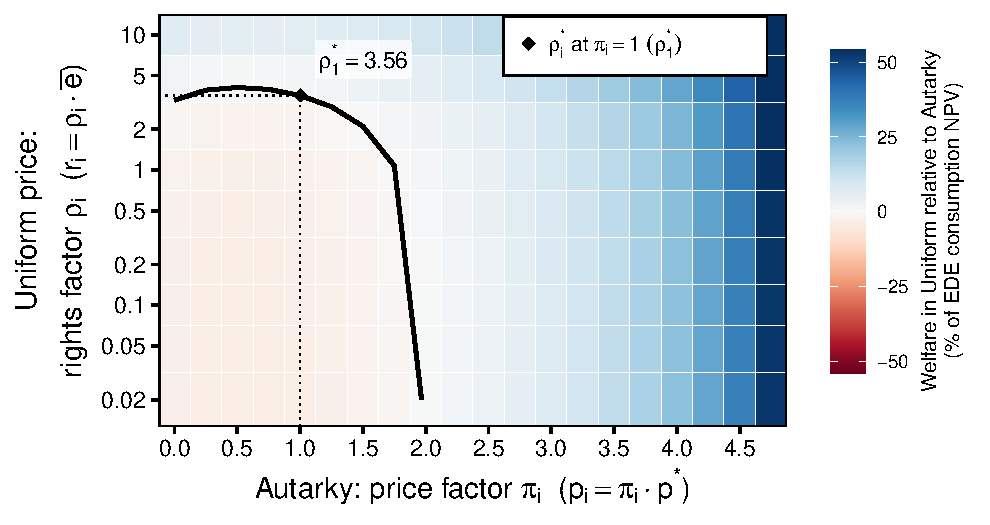
\includegraphics[width=\linewidth]{figures/heatmap_eqpc_USA.pdf}\caption{United States}\end{subfigure}\hfill
  \begin{subfigure}[b]{0.49\textwidth}\centering
    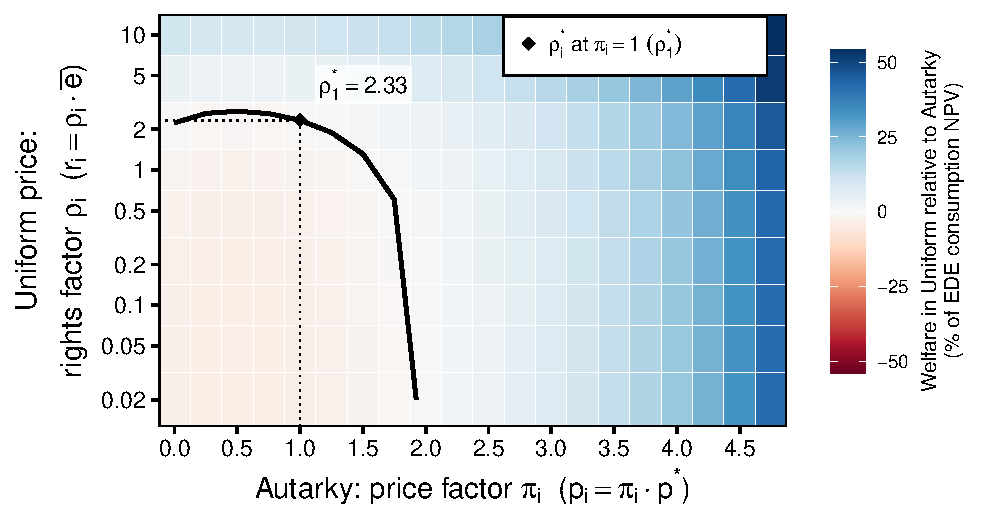
\includegraphics[width=\linewidth]{figures/heatmap_eqpc_RUS.pdf}\caption{Russia}\end{subfigure}\\[2pt]
  \begin{subfigure}[b]{0.49\textwidth}\centering
    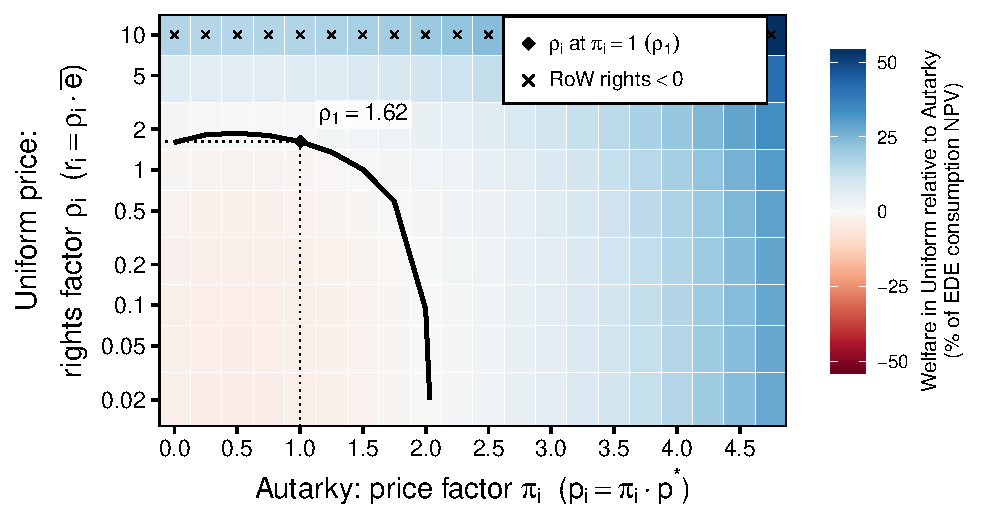
\includegraphics[width=\linewidth]{figures/heatmap_eqpc_CHN.pdf}\caption{China}\end{subfigure}\hfill
  \begin{subfigure}[b]{0.49\textwidth}\centering
    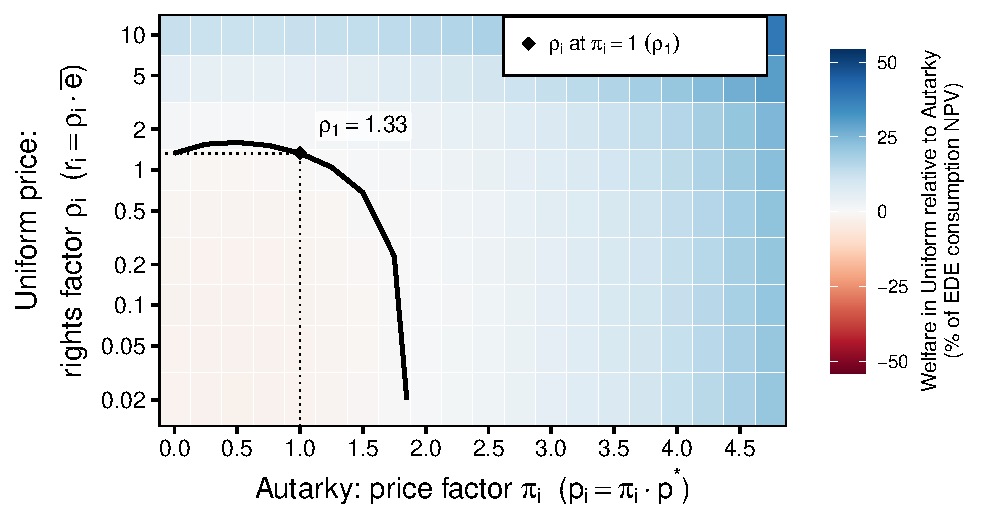
\includegraphics[width=\linewidth]{figures/heatmap_eqpc_TUR.pdf}\caption{Turkey}\end{subfigure}\\[2pt]
  \begin{subfigure}[b]{0.49\textwidth}\centering
    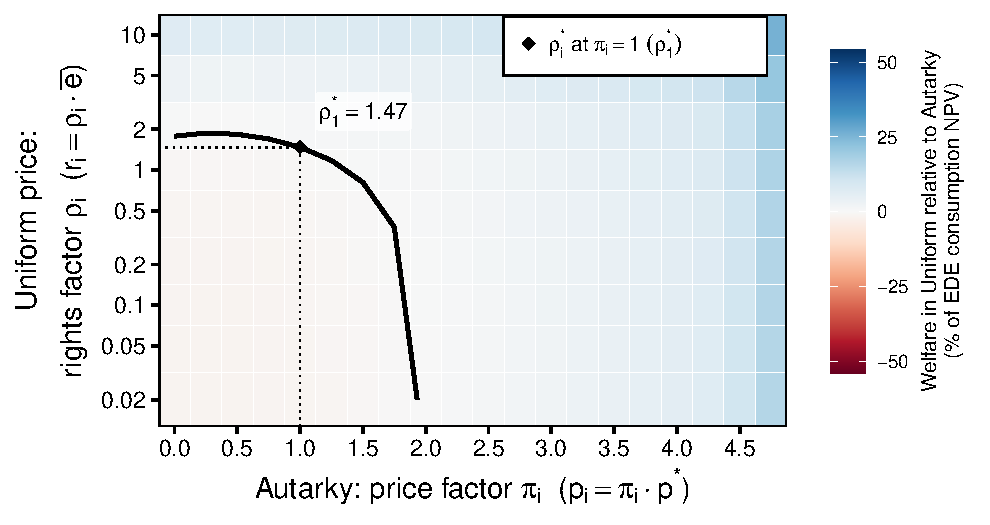
\includegraphics[width=\linewidth]{figures/heatmap_eqpc_EU27.pdf}\caption{European Union (EU27)}\end{subfigure}\hfill
  \begin{subfigure}[b]{0.49\textwidth}\centering
    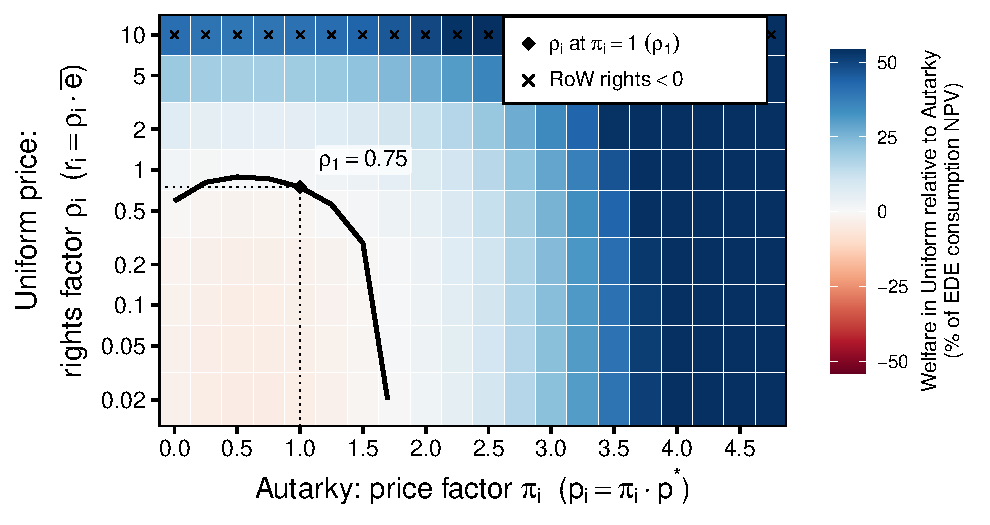
\includegraphics[width=\linewidth]{figures/heatmap_eqpc_IND.pdf}\caption{India}\end{subfigure}\\[2pt]
  \begin{subfigure}[b]{0.49\textwidth}\centering
    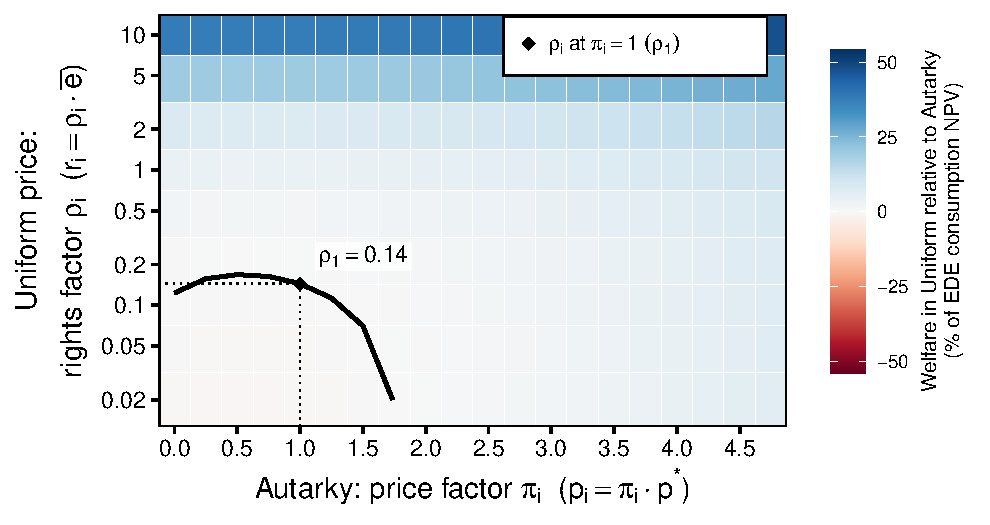
\includegraphics[width=\linewidth]{figures/heatmap_eqpc_NGA.pdf}\caption{Nigeria}\end{subfigure}\hfill
  \begin{subfigure}[b]{0.49\textwidth}\centering
    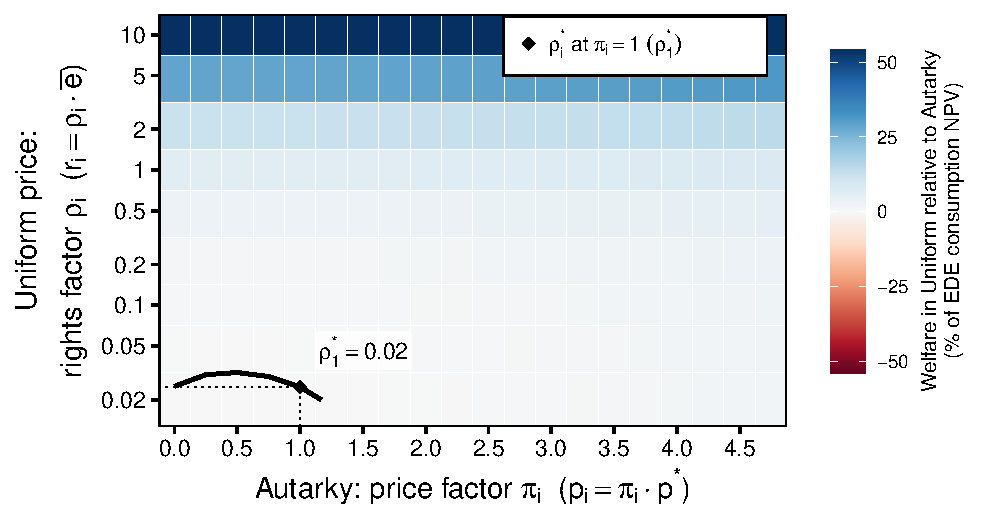
\includegraphics[width=\linewidth]{figures/heatmap_eqpc_COD.pdf}\caption{DR Congo}\end{subfigure}
  \caption{Welfare gain of the uniform-price regime over autarky, welfare variant.}
  \label{fig:heatmaps_eqpc}
  \begin{minipage}{\textwidth}\footnotesize\singlespacing
  \emph{Note}: As Figure~\ref{fig:heatmaps}, for the welfare variant: colours give the difference in the NPV of population-weighted equally-distributed-equivalent consumption over 2025--2100, in percent, clipped at $\pm54$ (the 95th percentile of the absolute difference), and the carbon revenue is returned as an equal per capita dividend within countries in both regimes. The indifference curve is traced from the equivalent allocation solved at each $\pi_i$ of the grid.
  \end{minipage}
\end{figure}}{}

The two variants differ through a within-country channel. In NICE, carbon costs fall on deciles in proportion to income raised to an elasticity below one, which is regressive; an equal per capita dividend more than offsets it, so that a carbon price, net of the dividend it funds, redistributes from richer to poorer deciles, which an inequality-averse criterion values. In the consumption variant, the revenue is returned in proportion to $c^{\eta}$ and the criterion ignores the distribution across deciles, so that channel is shut down.

\paragraph{Equivalent rights by country.} At $\pi_i=1$ the two variants give nearly the same allocations: $\rho_1$ is 3.56 for the United States, 1.62 for China, 1.47 for the EU27, 0.75 for India and 0.14 for Nigeria, within 0.07 of the consumption variant (Table~\ref{tab:summary}). Away from $\pi_i=1$ they differ. In both regimes the country returns its carbon revenue as an equal per capita dividend, so a domestic carbon price also redistributes from its richer to its poorer deciles, which the welfare criterion values. Compared with an unpriced autarky, the uniform-price regime thus brings the country that redistribution on top of the allocation, and fewer rights are needed to make it indifferent. As $\pi_i$ rises from zero, autarky brings the same redistribution, so the equivalent allocation rises; beyond $\pi_i\approx1$, abatement costs dominate and it falls. The equivalent allocation is therefore highest around $\pi_i=0.5$--$1$ rather than at a zero price: 4.08 at $\pi_i=0.5$ against 3.28 at $\pi_i=0$ for the United States, 0.17 at most against 0.12 at $\pi_i=0$ for Nigeria, and 0.03 at most for the DRC. The most that any non-negative price can offer a low emitter is therefore even smaller than in the consumption variant, which strengthens the conclusion of Section~\ref{sec:by_country}. This pattern reflects the absence, in the model, of any other instrument of within-country redistribution: a lump-sum redistribution would deliver the same welfare gain without abatement, so the carbon price is here valued in part as a redistributive device.

\paragraph{Equivalent rights of the proposals.} The surplus left by uniform pricing is far larger in the welfare variant (Table~\ref{tab:equiv_rights_benchmarks}). Converted into lower emissions, it reaches 27.0\% of the coalition's emissions under \citet{wolfram_building_2025}, 21.4\% under \citet{banerjee_grand_2025} and 28.5\% under Equal Right, against 4.8\%, 3.9\% and 13.4\% in the consumption variant. The equivalent allocations, which add up to these tighter caps, are accordingly lower, and the difference falls mostly on middle- and low-income members (India 0.58 against 0.92 under Banerjee et al., China 1.29 against 1.60), while high emitters keep similar allocations (the United States 2.58 against 2.51). Again, this is not a larger efficiency gain from uniform pricing.
The reduced-emissions cut of the welfare variant thus mixes the efficiency gain of uniform pricing with the within-country redistributive value of carbon revenue; the consumption variant isolates the former.

\clearpage
\section{The Equal Right schedule on its original price path}
\label{app:ede}

The Equal Right schedule is designed to rise by about 16\% a year, far faster than the 5\% we assume for the other two. Table~\ref{tab:equiv_rights_equalright} reports it on both paths. On its own path, the schedule pushes most members to full abatement by 2050 and reaches 1.48\textdegree C of warming; its coalition price is far above the other schedules', and its allocations are compressed towards an equal per capita share, the dividend of the global fund weighing more heavily the higher the price. The dividend of uniform pricing is larger still: replacing the schedule with the coalition price and the equivalent allocation cuts the coalition's emissions by 14.7\%, against 13.4\% on the 5\%-a-year path. Its effect on 2100 warming is smaller ($-0.010$\textdegree C against $-0.036$\textdegree C), because a schedule that has already driven emissions to zero by mid-century leaves little room for a further cut in cumulative terms.

\IfFileExists{../output/equivalent_rights_equalright_joint.tex}{%
\begin{table}[htbp]
\centering\small\singlespacing
\caption{The Equal Right schedule on its own escalation path and at 5\% a year.}
\label{tab:equiv_rights_equalright}
\resizebox{.9\textwidth}{!}{% Generated by src/equivalent_rights_proposals.jl (write_main_table) -- do not edit by hand.
\begin{tabular}{lcccc}
  \toprule
  & \multicolumn{2}{c}{\textbf{Equal Right}} & \multicolumn{2}{c}{\textbf{Equal Right, 5\%/yr}} \\
  \cmidrule(lr){2-3} \cmidrule(lr){4-5}
  \textbf{Country} & $p_{2030}$ & $\tilde\rho$ & $p_{2030}$ & $\tilde\rho$ \\
  \midrule
  Russia & 513 & 0.22 & 240 & 0.12 \\
  United States & 513 & $-$0.02 & 240 & $-$0.16 \\
  European Union (average) & 496 & 0.35 & 232 & 0.31 \\
  China & 231 & 1.11 & 108 & 1.13 \\
  Turkey & 231 & 0.96 & 108 & 0.99 \\
  Brazil & 231 & 0.77 & 108 & 0.78 \\
  Indonesia & 205 & 0.87 & 96 & 0.91 \\
  India & 90 & 1.10 & 42 & 1.17 \\
  Nigeria & 90 & 0.76 & 42 & 0.76 \\
  DR Congo & 32 & 0.67 & 15 & 0.68 \\
  \midrule
  \multicolumn{5}{l}{\textit{Reduced emissions: every member as well off as under the proposal (ignoring avoided damages)}} \\
  World temp.~2100, change (\textdegree{}C) &  & $-$0.010 &  & $-$0.036 \\
  Emissions change in the coalition (\%) &  & $-$14.7\% &  & $-$13.4\% \\
  Post-damage consumption gain (\%) &  & 0.035\% &  & 0.095\% \\
  \midrule
  \multicolumn{5}{l}{\textit{Increased consumption: coalition emissions as under the proposal}} \\
  Coalition consumption gain (in \%) &  & 0.097\% &  & 0.189\% \\
  \bottomrule
\end{tabular}
}
\begin{minipage}{\textwidth}\footnotesize\singlespacing
\emph{Note}: As Table~\ref{tab:equiv_rights_main}, for the Equal Right schedule of price floors grown at its own rate (about 16\% a year) and at the 5\% a year assumed for the other schedules. Both are run with the proposal's global fund: the revenue of every country is pooled and returned as an equal per capita dividend to the world population.
\end{minipage}
\end{table}}{}

\end{document}
